\documentclass[letterpaper,12pt,onehalfspacing,twoside]{article}

\usepackage{lipsum,kantlipsum}
%\usepackage{times}
\usepackage[tmargin=1in,bmargin=1in,lmargin=1in,rmargin=1in]{geometry}
\usepackage{setspace}
%  \spacing{1.5}
\usepackage{float}
\setlength{\parindent}{0pt}
\setlength{\parskip}{1em}
% \setlength{\parskip}{\baselineskip}

\usepackage{verbatim}
\usepackage{titlesec}
% \usepackage{xcolor}
\usepackage[	pdfauthor={Jay R. Shah},
			pdftitle={Demand risk management in clustered vehicle routing}]{hyperref}
\usepackage{color}
 \definecolor{darkblue}{rgb}{0.0,0.0,0.3}
 \definecolor{lighterblue}{rgb}{0.0,0.0,0.6}
 \definecolor{shade}{gray}{0.8}
 \hypersetup{colorlinks,breaklinks,
            linkcolor=black,urlcolor=darkblue,
            anchorcolor=lighterblue,citecolor=lighterblue}

\usepackage{tikz}
\usetikzlibrary{calc}
\usepackage{eso-pic}
% \usepackage{background}
\usepackage{pdflscape}

\usepackage{titling}
\setlength{\droptitle}{-10em}   % This is your set screw

\usepackage{tfrupee} % Rupee symbol

\usepackage{graphicx}
\usepackage{amsmath} % [fleqn] for left justified % to have only a few equations left justified, crude way is to use \phantom{\hspace{<length>}}
 %\setlength{\mathindent}{0pt} % after the equation. % OR better use what is shown in Chapter8.
\usepackage{amssymb}
% \usepackage{gensymb}
\usepackage[shortlabels]{enumitem}
\usepackage{chemfig}
\usepackage[version=3]{mhchem} % Package for chemical equation typesetting
\usepackage{textcomp}
\usepackage{amsthm} % for theorem-like settings
\usepackage{mathrsfs} % math alphabets

\usepackage{longtable}
\usepackage{caption}
%\usepackage{subfigure}
\usepackage{subfig} % causing problems
\usepackage{tabularx}
\usepackage{decorule}
\usepackage{booktabs} % Allows the use of \toprule, \midrule and \bottomrule in tables for horizontal lines
\usepackage{multirow}
\usepackage{bigstrut}
\usepackage{chngcntr}

\usepackage[titletoc,title]{appendix} % remove titletoc, add toc for another (acceptable??) way of presenting appendices in toc

% \usepackage[nottoc]{tocbibind} %% get NOT numbered bibliography in toc. write [nottoc,numbib] to make it numbered

%\usepackage{tocloft}
%\renewcommand{\printtoctitle}{\centering\Huge\bfseries}
\renewcommand{\contentsname}{\centering \textbf{Table of Contents}}

%% ------------------------HEADER FOOTER SETTINGS------------------------------------------------------------------------------------------------------------

\usepackage{fancyhdr}
\pagestyle{fancy}

%\renewcommand{\sectionmark}[1]{%
% \markright{\thesection\ #1}}
\renewcommand{\sectionmark}[1]{\markright{\thesection.\quad #1}}
\renewcommand{\subsectionmark}[1]{} % eliminates subsection names from headers
\fancyhf{} 
\fancyfoot[RO,LE]{\thepage}
%\fancyfoot[LO,RE]{\it Design a plant to manufacture 500 TPA of N-Methyl J Acid}
\fancyhead[C]{\it\nouppercase\rightmark} % 1. section name

\renewcommand{\headrulewidth}{0pt}
\renewcommand{\footrulewidth}{0pt}
%\addtolength{\headheight}{0.5pt} 
%\fancypagestyle{plain}{%
%\fancyhead{}
%\renewcommand{\headrulewidth}{0pt} % and the line
%}

%% -------------------------THEOREM-LIKE ENVIRONMENT--------------------------------------------------------------------------------------------------------

% \theoremstyle{definition}
% \newtheorem{msdssection}{Section}

\newtheoremstyle{msds} 	          % name
    {\topsep}                    	          % Space above
    {\topsep}                    	          % Space below
    {\normalfont}                           % Body font
    {}                           	          % Indent amount
    {\bfseries\large}                      % Theorem head font
    {.}                          	          % Punctuation after theorem head
    {.5em}                       	          % Space after theorem head
    {}  				          % Theorem head spec (can be left empty, meaning ‘normal’)

\theoremstyle{msds}
\newtheorem{msdssection}{Section}
%  \counterwithin*{msdssection}{subsection}

%% amsthm package documentation for more settings: http://ctan.imsc.res.in/macros/latex/required/amscls/doc/amsthdoc.pdf

%%----------RESET THEOREM COUNTER AFTER EACH \subsection--------------------------------------------------------------------------------------------

\makeatletter
  \@addtoreset{msdssection}{subsection}
\makeatother

%% ------------------------SECTION ALIGNMENT--------------------------------------------------------------------------------------------------------------------




\titleformat*{\section}{\large\bf} % the \titleformat* is short form version. \titleformat gives error because it takes 7 arguments.
\titleformat*{\subsection}{\normalfont\bf}
\titleformat*{\subsubsection}{\normalfont\bf}
% \titleformat*{\subsubsubsection}{\normalfont\bf}

\titlespacing\section{0pt}{0pt plus 0pt minus 2pt}{0pt plus 0pt minus 2pt}
\titlespacing\subsection{0pt}{0pt plus 0pt minus 2pt}{0pt plus 0pt minus 2pt}
\titlespacing\subsubsection{0pt}{0pt plus 0pt minus 2pt}{0pt plus 0pt minus 2pt}

%\titlespacing{\section}{0pt}{\parskip}{-\parskip}
%\titlespacing{\subsection}{0pt}{\parskip}{-\parskip}
%\titlespacing{\subsubsection}{0pt}{\parskip}{-\parskip}

% \setcounter{secnumdepth}{3} % levels under \subsubsection are not numbered
\setcounter{tocdepth}{3}    % levels under \subsubsection are not listed in the TOC

%% -----------------------------------------DEFINE NEW LIST(S)----------------------------------------------------------------------------------------------------------

\newlist{tinylist}{itemize}{3}
    \setlist[tinylist]{label=\textbullet,
			leftmargin=*,
			parsep=0pt,
			topsep=0pt,
			partopsep=0pt,
			itemsep=0pt}

\newlist{smalllist}{itemize}{3}
    \setlist[smalllist]{label=\textbullet,
			leftmargin=*,
			parsep=2pt,
			topsep=0pt,
			partopsep=0pt,
			itemsep=0pt}

%% ----------------------------------------------------------------------------------------------------------------------------------------------------------------------------

%\usepackage[backend=bibtex,url=false,doi=false,isbn=false,style=authoryear,natbib=true]{biblatex} % Uses the bibtex backend with the authoryear citation style (which resembles APA)
% \usepackage[backend=bibtex,url=false,doi=false,isbn=false,style=numeric-comp,sorting=none]{biblatex} % exclude (include) using doi=false (true)

\usepackage{natbib} % [numbers] to get numbers
\usepackage{notoccite}

%\addbibresource{homepaperbib.bib} %% uncomment biblatex package
% \bibliography{Seminar.bib} %% uncomment biblatex package

%% ------------------------------------------------------------------------------------------------------------------------------------------------------
\allowdisplaybreaks
\begin{document}

\pagestyle{plain}

\begingroup  
  \centering
  \LARGE Demand risk management in clustered vehicle routing
  \\ \large 06-815 Course Project - Proposal\\
  \large Jay Shah - jrshah@andrew.cmu.edu\par
\endgroup


Vehicle routing problems (VRPs) and their extensions constitute some of the most studied problems in combinatorial optimization and operations research. In general terms, the VRP aims to define routes of vehicles to fulfill the service demands of customers placed at known locations.  This group of problems has extensive scope of applications, such as transportation, network optimization, supply chain and distribution planning, etc. The capacitated vehicle routing problem (CVRP), first described by \cite{dantzig}, is concerned with the minimum cost delivery of a single product from a depot to customers through a specified number of capacity-constrained vehicles.

The Generalized Vehicle Routing Problem (GVRP) is a generalization of the CVRP in which nodes (customers) are partitioned into mutually exclusive and exhaustive node sets, called clusters \citep{POP201297}. We are interested in finding optimal routed from the given depot to the number of predefined clusters which include exactly one node from each cluster.

\textbf{Motivation}

The classical GVRP is a deterministic optimization problem because it assumes that the customer demands are known with certainty ahead of planning the route. However, there are many real life scenarios where this is not the case. Consider the distribution of goods by sea to a number of customers situated in an archipelago as in Philippines, New Zealand, Indonesia, Italy, etc. A number of potential harbors is selected for each island and a fleet of ships is required to visit one harbor for every island. Goods from the ships are unloaded based on a demand which is realized when the ship visits reaches the island. As such, a decision has to be made when at the depot in regards to the amount of goods to be loaded at the beginning of the route. Since the cost of the route could be directly influenced by the amount of loaded goods, it is desirable to ensure that the minimum amount is loaded while satisfying all customer demands.

Another variant of the CVRP is the clustered capacitated vehicle routing problem (CCVRP). The customers are organized into clusters, similar to the GVRP. However, instead of visiting exactly one customer from each cluster, the vehicle must satisfy demands by visiting all the customers in a cluster consecutively. A potential application of this problem is the routing of fuel trucks to gas stations. Demand uncertainty in this case arises due to variability in the amount of unsold fuel available at the gas station from the previous delivery. It is of interest to minimize the amount of fuel transported by the fuel truck for safety and cost reasons.
Mail pickup and delivery in a multi-storey or multi-pavilion office complex is a similar application of the CCVRP \citep{laporteandpalekar}. Examples of the GVRP and CCVRP are shown in Fig. \ref{fig:example_gvrp} and \ref{fig:example_ccvrp} respectively.

\textbf{Current state of the art}

Mathematical programming approaches to these type of problems have so far focused on deterministic scenarios i.e. when customer demand and costs are known in advance. Both exact \citep{bektasKara, POP201297} and metaheuristic approaches \citep{Noon, GHIANI200011,  doi:10.1063/1.3130618} have not considered uncertainty scenarios which arise in real life situations. The objective of future work should therefore be the development of a comprehensive framework to handle uncertainty and risk in various parameters involved in capacitated vehicle routing with customers grouped into clusters.

\begin{figure}[!tbp]
  \centering
  \begin{minipage}[b]{0.49\textwidth}
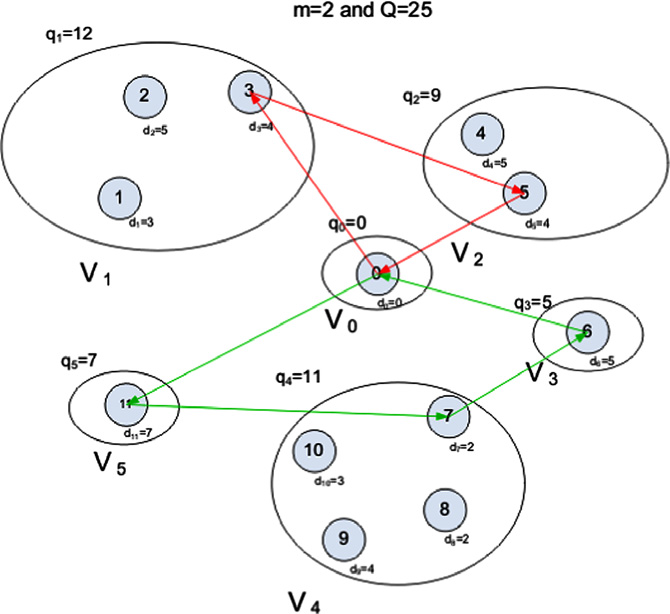
\includegraphics[width=\textwidth]{example_gvrp.png}
\caption{An example of a GVRP and a feasible solution \citep{POP201297}}
\label{fig:example_gvrp}
  \end{minipage}
  \hfill
  \begin{minipage}[b]{0.49\textwidth}
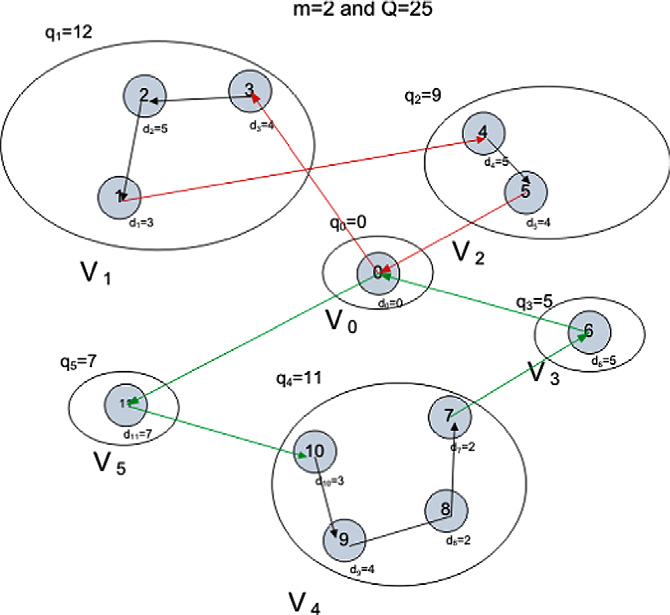
\includegraphics[width=\textwidth]{example_ccvrp.png}
\caption{An example of a CCVRP and a feasible solution \citep{POP201297}}
\label{fig:example_ccvrp}
  \end{minipage}
\end{figure}

Mitigating risk involves designing feasible routes that ensure that all possible realizations of uncertain parameters are accounted for, while minimizing the cost or other objective function. Robust optimization (RO) assumes that the uncertain data lies in a so-called ``Uncertainty set''. Constraint violation is not allowed for any realization of data in the uncertainty set. RO results is a static, ``here-and-now'' solution that is often overly conservative. Adjustable RO \citep{gorissen} on the other hand results in a more flexible solution policy by adjusting future decisions based on the actual realizations of the uncertain parameters as they occur.

Hence the objective of the proposed work is the development of a comprehensive framework for both static and adjustable robust optimization for the mitigation of demand and cost risk in generalizations of CVRPs defined above. The definition of the uncertainty set is heavily dependent on past data. Past customer demand data can be used to describe either discrete or continuous uncertainty sets. MILP formulations previously described in literature \citep{POP201297, bektasKara} can be reformulated to ensure tractability with the RO frameworks.

\textbf{Preliminary results}

Preliminary studies conducted to compare exact formulations for the GVRP indicate that a modern flow-based formulation described by \citep{POP201297} exhibits sufficient LP relaxation tightness to be able to solve deterministic problems of up to 70 customers to optimality with sufficient efficiency. Other formulations such as the node-based one described by the same authors and one by \citep{bektasKara} exhibit significantly higher difficulty to solve to optimality.






%\begin{figure}[htbp]
%\centering
%\end{figure}
%
%\begin{figure}[htbp]
%\centering
%\end{figure}
%\textbf{Definition of the GVRP}
%
%\textbf{Potential sources of demand risk}
%
%\textbf{Potential uncertainty sets}
%
%\textbf{Solution methods for deterministic problems}
%
%Several exact as well as metaheuristic algorithms have been proposed for the GVRP.
%
%The first mixed integer linear formulation of the GVRP was presented by \cite{bektasKara}, with a polynomially increasing number of binary variables and constraints. \cite{POP201297} presented two different formulations based on the additional auxiliary decision variables. These are called \emph{node-based} and \emph{flow-based} formulations respectively. The node-based formulation is structurally similar to the formulation by \cite{bektasKara}, but with stronger lower bounds. The flow-based formulation is completely new. In this section, a general semi-closed formulation for the GVRP is first presented and followed by the two formulations proposed by \cite{POP201297}.
%
%
%
%\textbf{Generation of additional test examples}
%
%Three additional test examples were generated using capactitated vehicle routing problem (CVRP) data obtained from CVRPLIB (\url{http://vrp.atd-lab.inf.puc-rio.br}). Instances \texttt{P-n50-k10}, \texttt{A-n69-k9} and \texttt{P-n76-k5} were chosen. The clusters were obtained by implementation of a simple clustering algorithm (K-means), with the number of clusters chosen such that the number of customers in any cluster is no more than 5. The demand of each cluster was calculated by summing the demands of each customer in that cluster. 
%Details of each of the problems under consideration is given in Table \ref{tab:problemdetails}.
%
%\textbf{Computational study}
%
%Both node-based and flow-based formulations described above were implemented in CPLEX and solved using a Windows PC with an Intel i7 processor (2.90 GHz). 
%
%\textbf{Tightness of root node relaxation}
%
%\begin{table}[htbp]
%\centering
%\caption{Deviation between root node relaxation and optimal values}
%\label{tab:rootnode}
%\begin{tabular}{@{}ccccc@{}}
%\toprule
%\textbf{Instance}              & \textbf{\begin{tabular}[c]{@{}c@{}}Best known\\  objective\end{tabular}} & \textbf{Formulation} & \textbf{\begin{tabular}[c]{@{}c@{}}Root node\\   relaxation\end{tabular}} & \textbf{\% Deviation} \\ \midrule
%\multirow{2}{*}{\texttt{GVRP1}}          & \multirow{2}{*}{527.813}     & flow                 & 498.594                        & 5.54                  \\
%                               &                              & node                 & 449.358                       & 14.86                 \\ \midrule
%\multirow{2}{*}{\texttt{GVRP2}}         & \multirow{2}{*}{557.564}     & flow                 & 533.9                       & 4.24                  \\
%                               &                              & node                 & 545.365                       & 2.19                  \\ \midrule
%\multirow{2}{*}{\texttt{P-n50-k10}} & \multirow{2}{*}{417.742}     & flow                 & 384.597  & 7.93                  \\
%                               &                              & node                 & 338.098                       & 19.07	  \\ \midrule
%\multirow{2}{*}{\texttt{A-n69-k9}}  & \multirow{2}{*}{756.131}     & flow                 & 692.212 & 8.45                  \\
%                               &                              & node                 & 560.44                       & 25.88 \\ \midrule
%\multirow{2}{*}{\texttt{P-n76-k5}}  & \multirow{2}{*}{500.955}     & flow                 & 450.746                       & 11.27                 \\
%                               &                              & node                 & 399.788                        & 21.30                 \\ \bottomrule
%\end{tabular}
%\end{table}
%
%Table \ref{tab:rootnode} shows a comparision between the root node relaxations for the flow- and node-based formulations. In all but one of the instances under consideration, the flow-based formulation shows a tighter LP lower bound. Thus we would expect the flow-based formulation to be more efficient than the node-based formulation. 
%
%This is indeed the case as seen in Table \ref{tab:compstudy}: the flow-based formulation finds a better objective value or closes the relative gap more than the node-based formulation. A one hour time limit for each problem was set for each of these calculations. Both formulations found the proven optimum within the time limit only for \texttt{GVRP2}. For \texttt{GVRP1}, only the flow-based formulation reached zero gap in 85 seconds. In all the other instances, the realtive gap at time limit was significantly smaller for the flow-based formulation.
%
%\begin{table}[htbp]
%\centering
%\caption{Model comparision for GVRP instances (time limit = 1 hour)}
%\label{tab:compstudy}
%\begin{tabular}{@{}cccccc@{}}
%\toprule
%\textbf{Instance}              & \textbf{Formulation} & \textbf{Status} & \textbf{\begin{tabular}[c]{@{}c@{}}Objective\\   value\end{tabular}} & \textbf{\begin{tabular}[c]{@{}c@{}}Relative gap\\   (\%)\end{tabular}} & \textbf{\begin{tabular}[c]{@{}c@{}}Number \\ of constraints\end{tabular}} \\ \midrule
%\multirow{2}{*}{\texttt{GVRP1}}         & flow                 & Optimal         & 527.813            & 0.01                       & 2108                 \\
%                               & node                 & Feasible        & 527.813            & 5.42                       & 1482                 \\ \midrule
%\multirow{2}{*}{\texttt{GVRP2}}         & flow                 & Optimal         & 557.564            & 0.00                       & 1242                 \\
%                               & node                 & Optimal         & 557.564            & 0.00                       & 952                  \\ \midrule
%\multirow{2}{*}{\texttt{P-n50-k10}} & flow                 & Feasible        & 417.742            & 0.75                       & 3094                 \\
%                               & node                 & Feasible        & 417.742            & 14.69                      & 2132                 \\ \midrule
%\multirow{2}{*}{\texttt{A-n69-k9}}  & flow                 & Feasible        & 756.131            & 1.25                       & 3385                 \\
%                               & node                 & Feasible        & 763.045            & 18.59                      & 2360                 \\ \midrule
%\multirow{2}{*}{\texttt{P-n76-k5}}  & flow                 & Feasible        & 508.194            & 6.04                       & 4896                 \\
%                               & node                 & Feasible        & 595.149            & 31.20                      & 3374                 \\ \bottomrule
%\end{tabular}
%\end{table}
%
%\begin{figure}[htbp]
%\centering
%\subfloat[Customer clusters]{%
%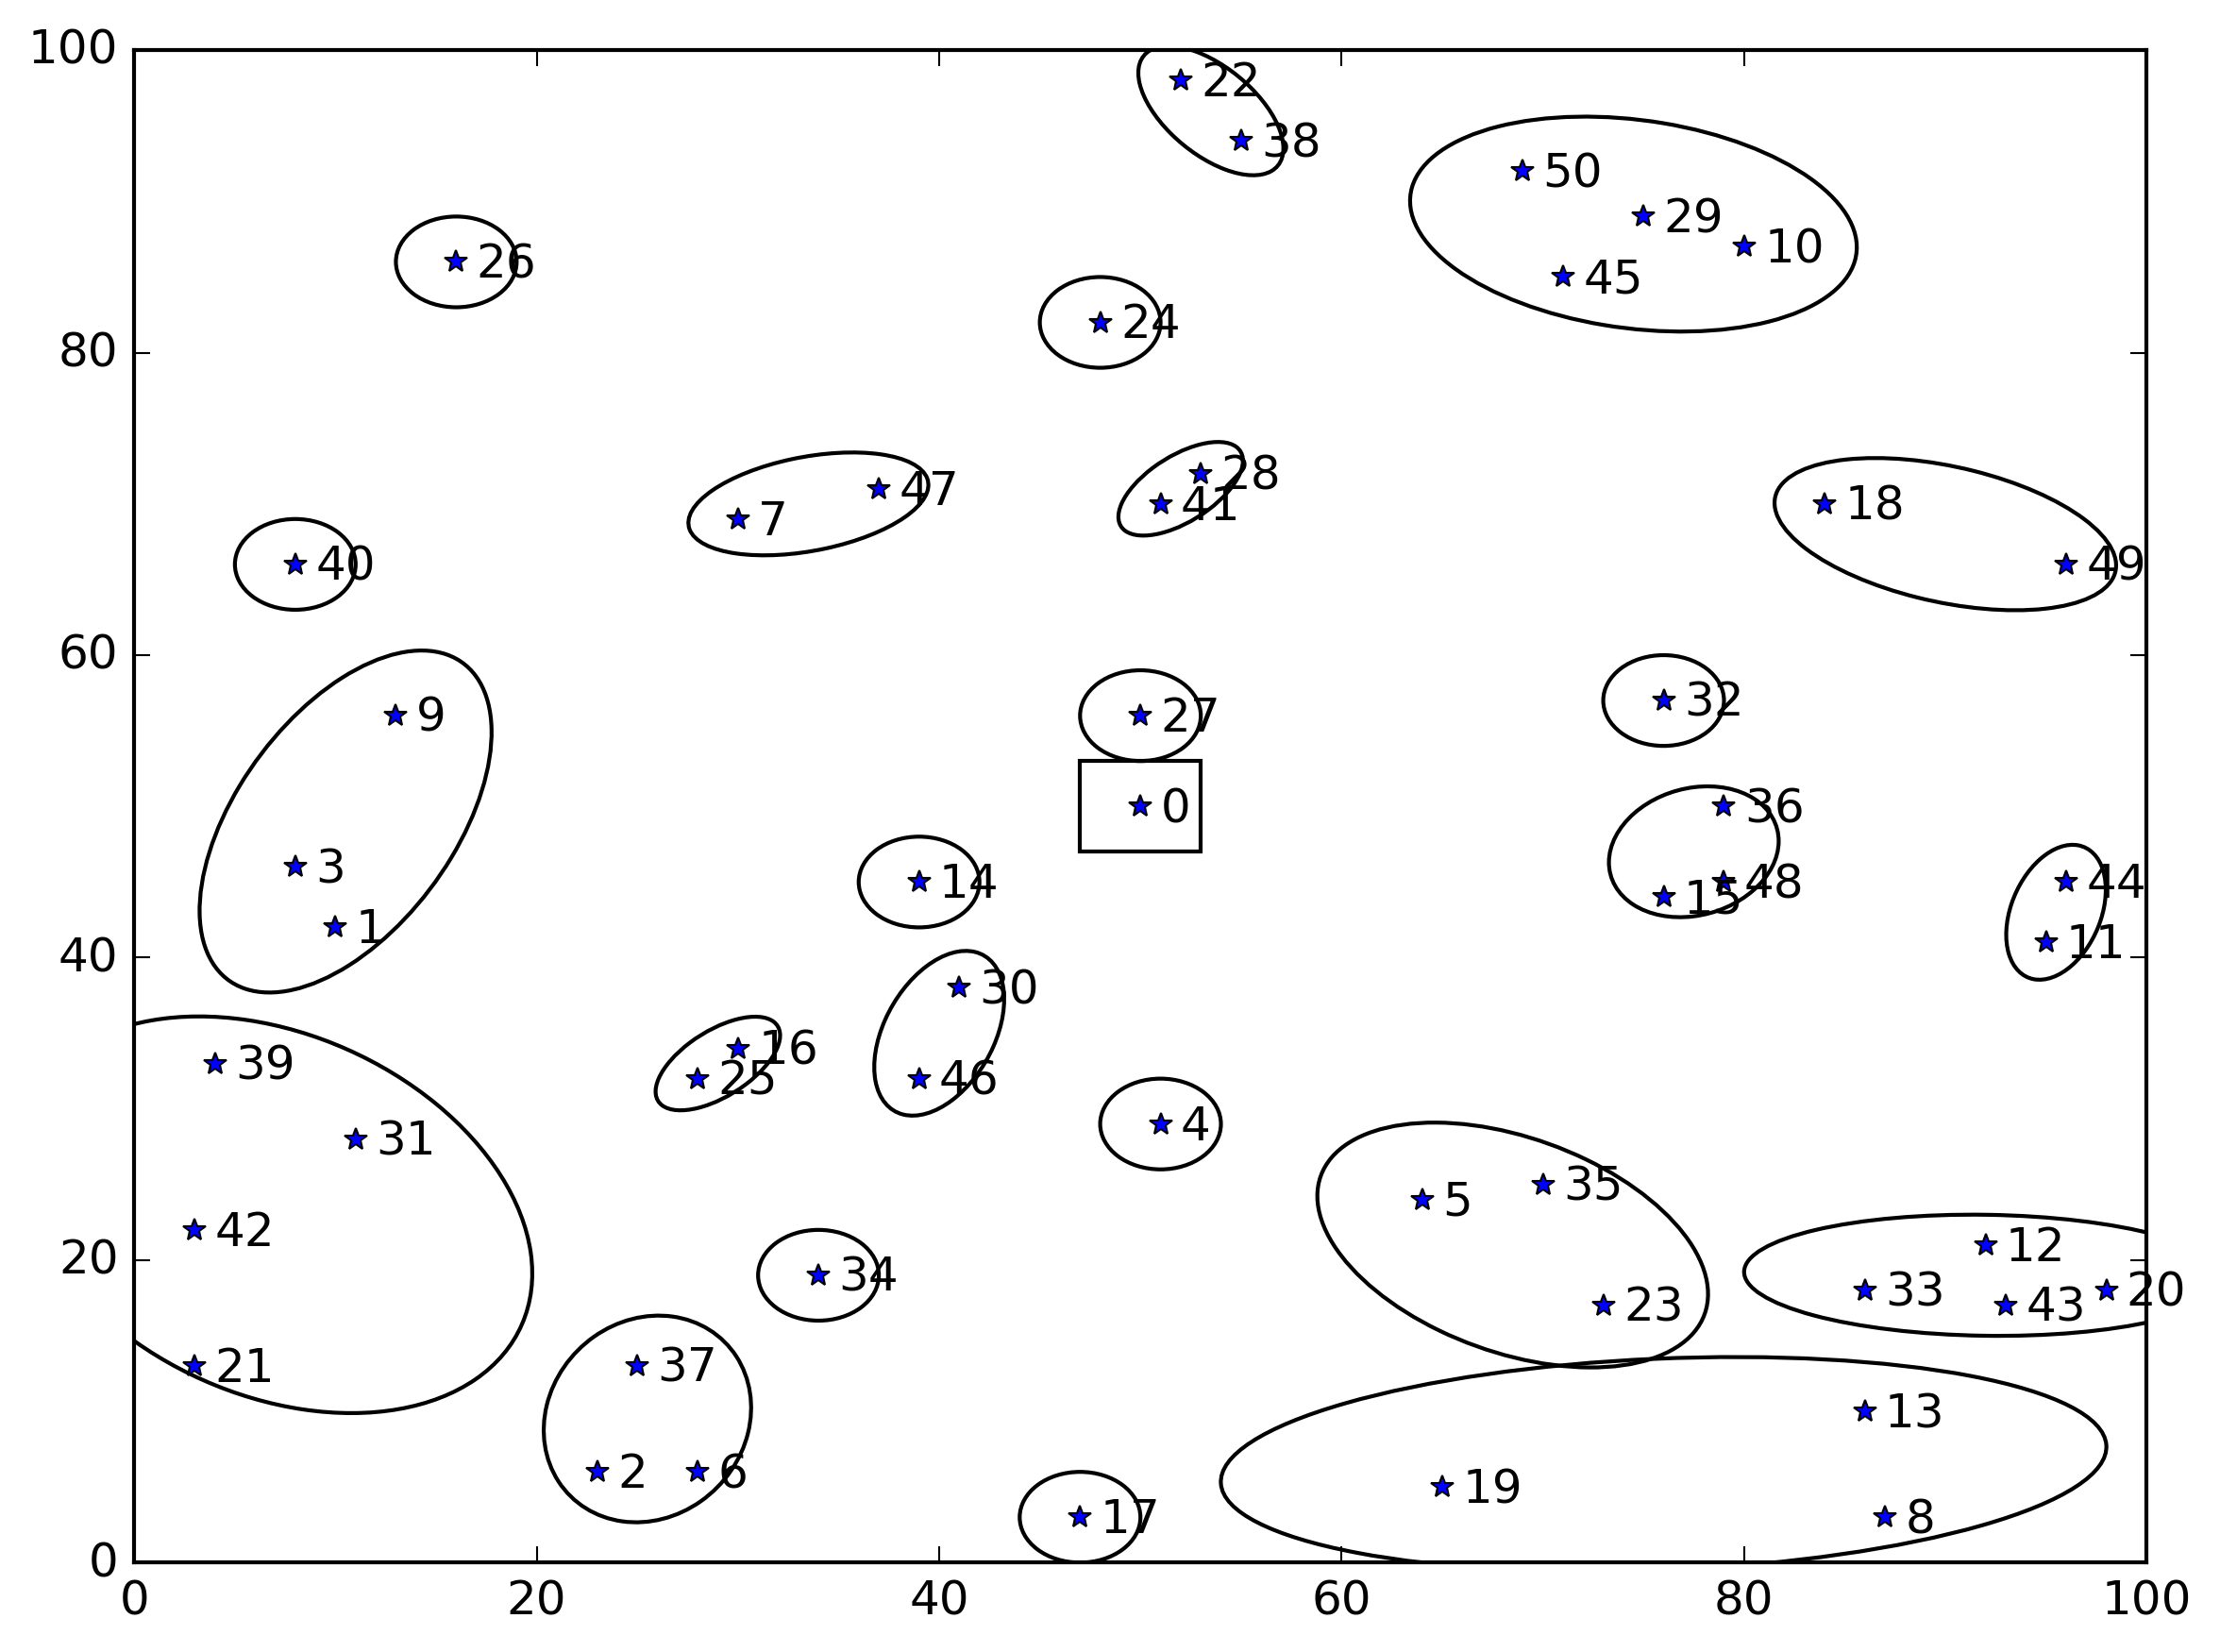
\includegraphics[width=0.45\textwidth]{GVRP_map.png}
%\label{fig:plot_11}}
%\quad
%\subfloat[Optimum solution (objective = 527.813)]{%
%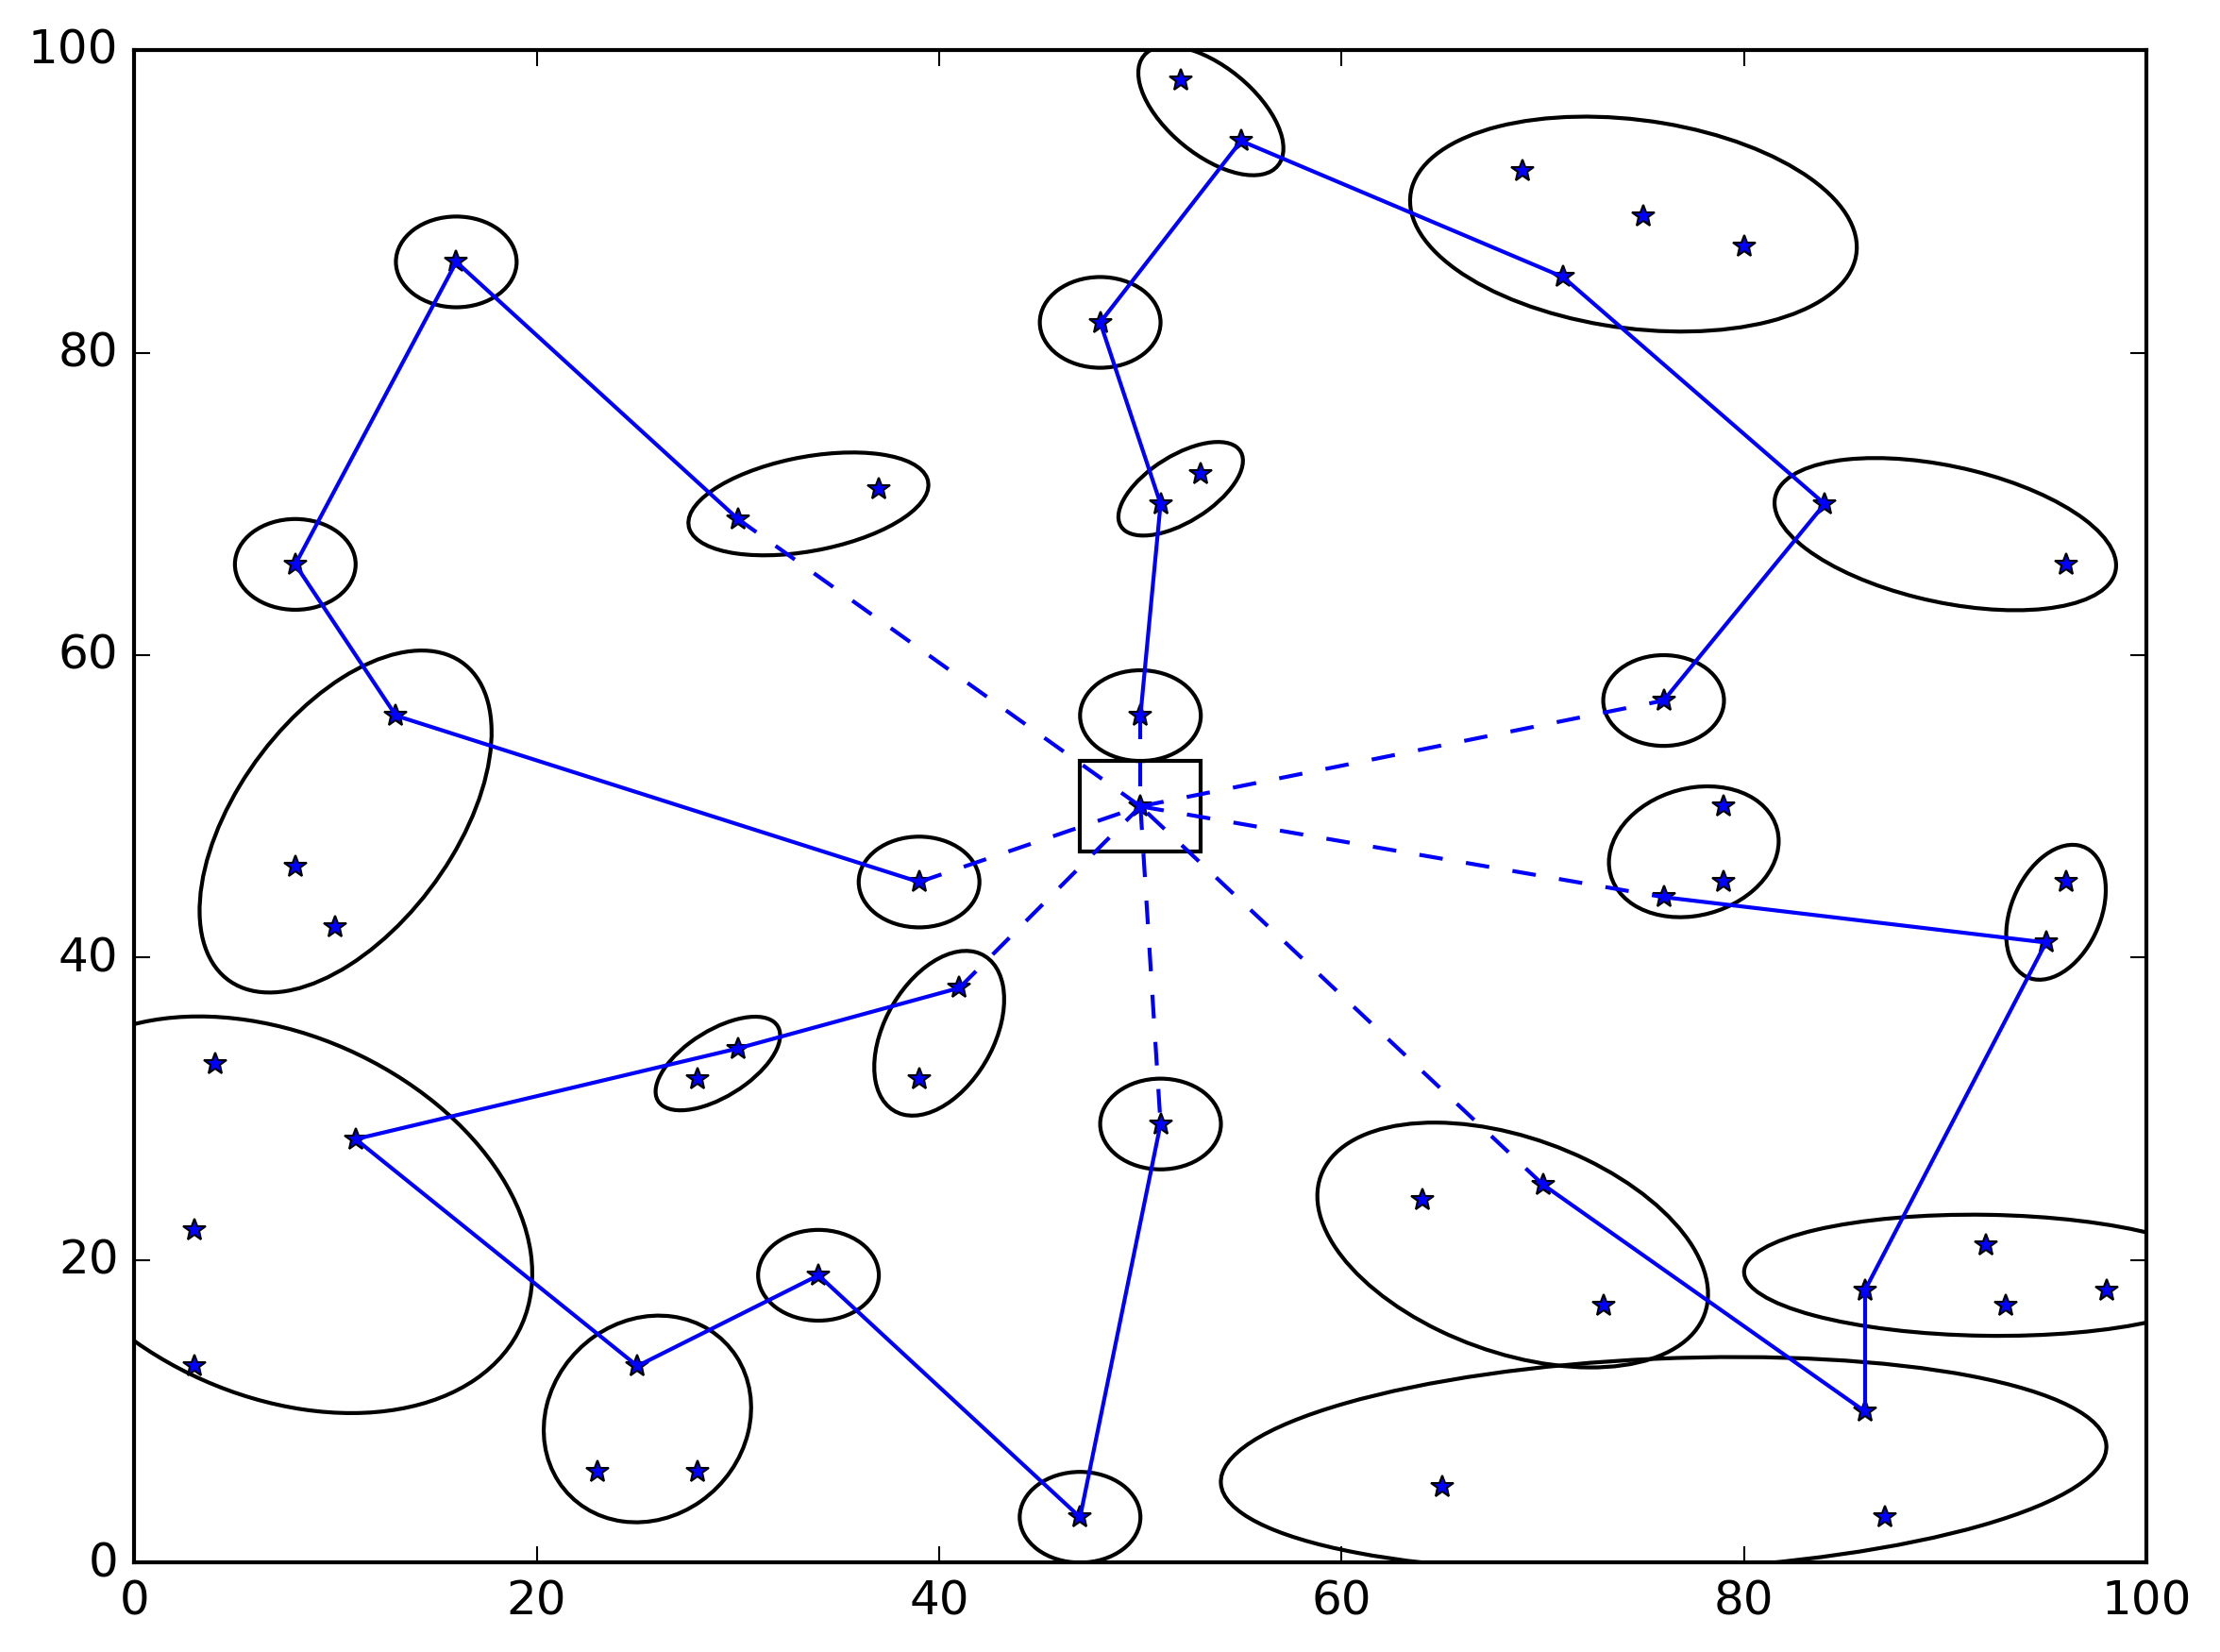
\includegraphics[width=0.45\textwidth]{GVRP_flow_n51_k25_m4_Q15_TL60_map.png}
%\label{fig:plots_12}}
%\caption{\texttt{GVRP1}}
%\label{fig:GVRP1sol}
%\end{figure}
%
%\begin{figure}[htbp]
%\centering
%\subfloat[Customer clusters]{%
%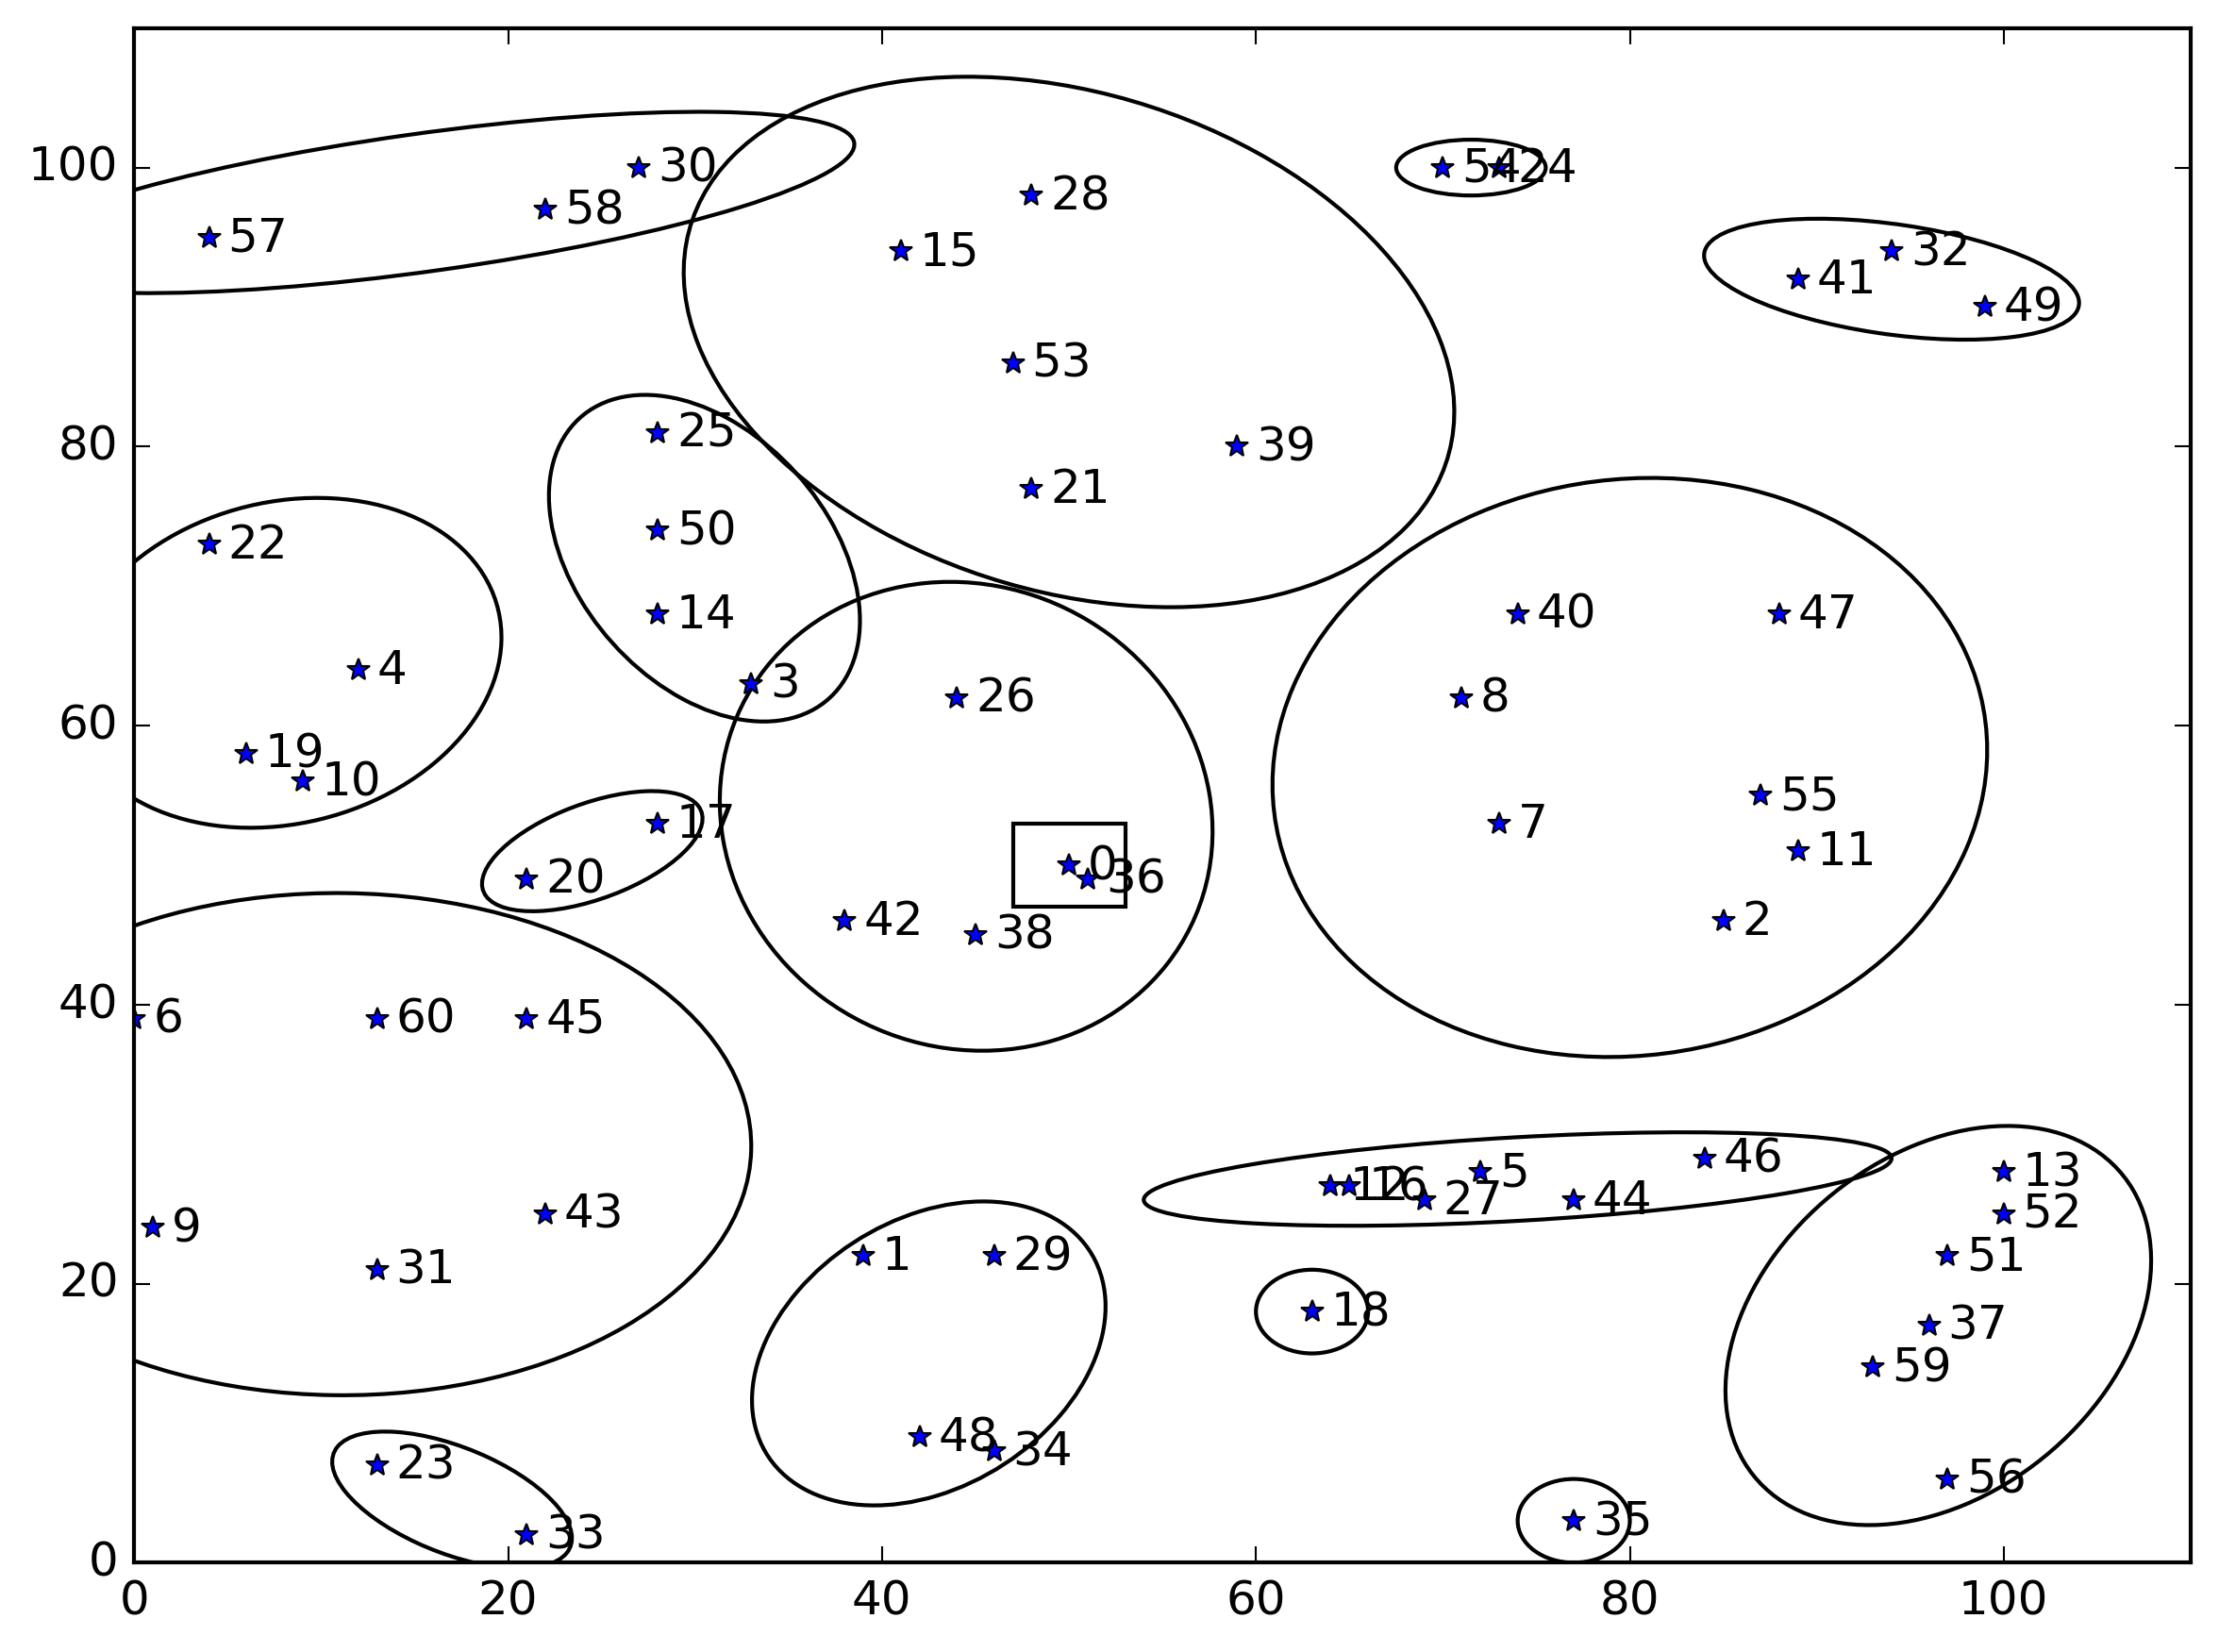
\includegraphics[width=0.45\textwidth]{GVRP2_map.png}
%\label{fig:plot_11}}
%\quad
%\subfloat[Optimal solution (objective = 557.564)]{%
%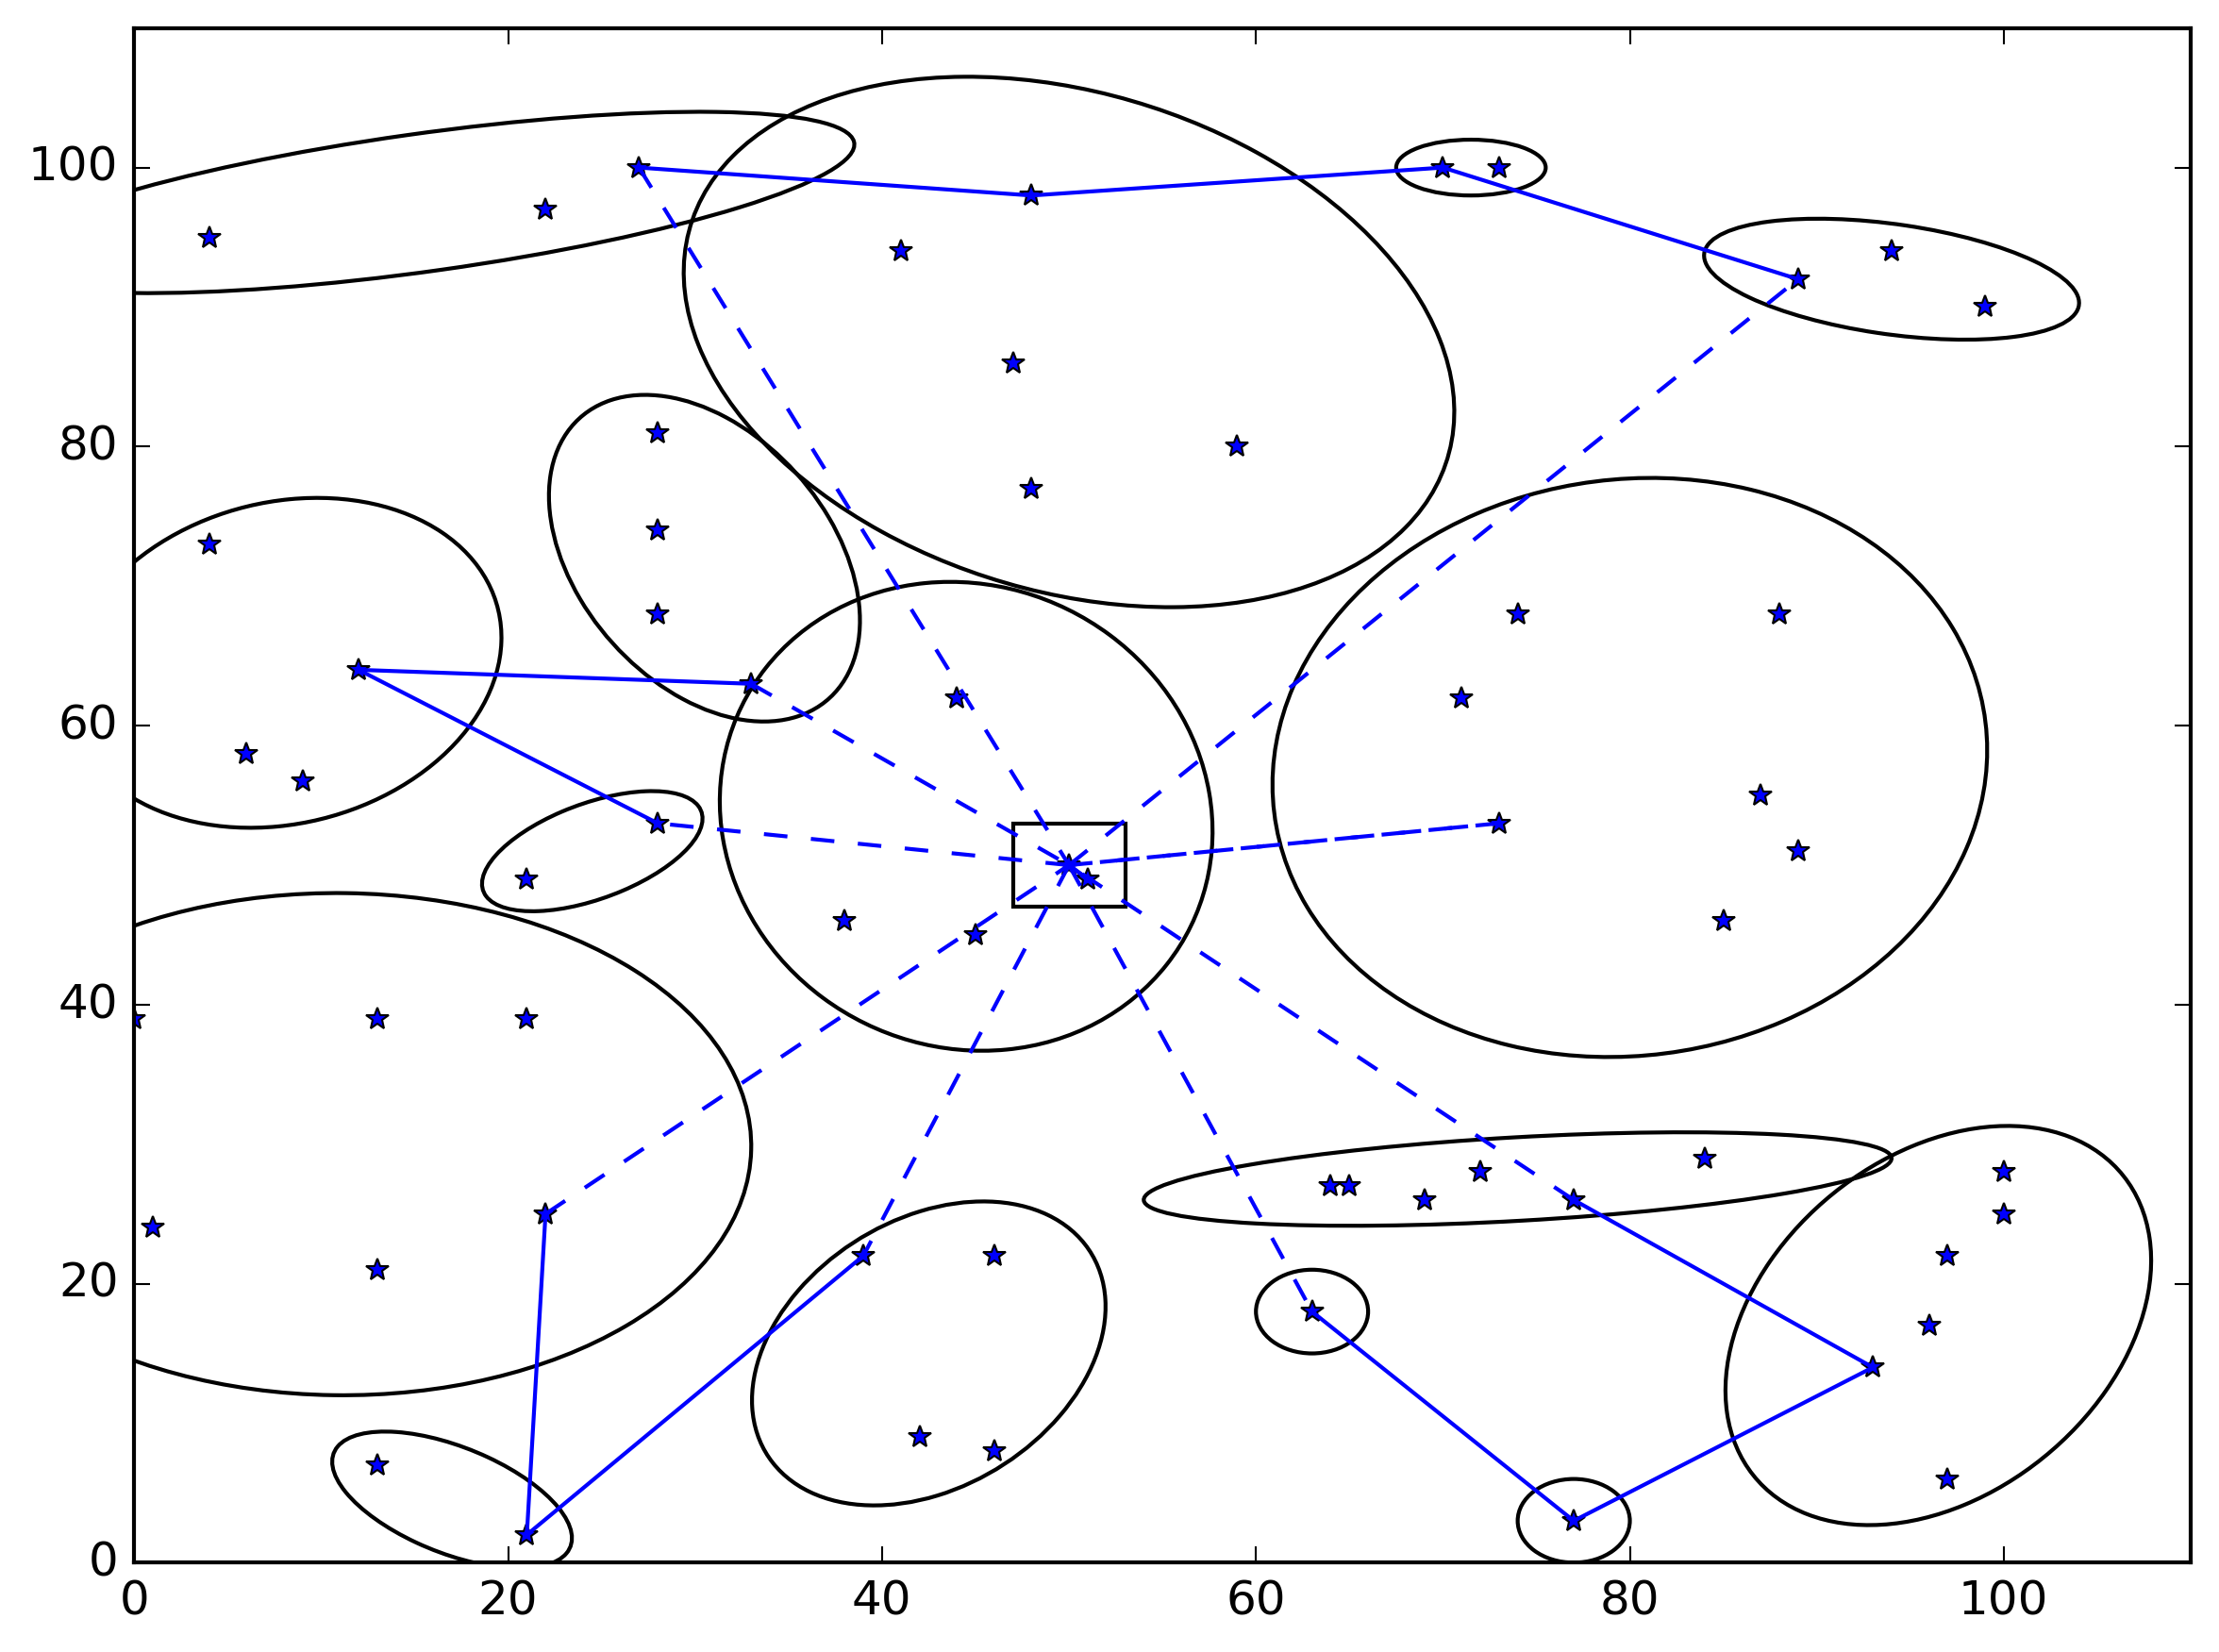
\includegraphics[width=0.45\textwidth]{GVRP2_flow_n61_k17_m6_Q15_TL10_map.png}
%\label{fig:plots_12}}
%\caption{\texttt{GVRP2}}
%\label{fig:GVRP2sol}
%\end{figure}
%The obtained objective value for \texttt{GVRP1} (Fig. \ref{fig:GVRP1sol}) is the same as the optimum reported by \cite{POP201297}. Since different constraints were used for \texttt{GVRP2}, the obtained solution does not match that reported by \cite{bektasKara}.
%
%Instances \texttt{P-n50-k10} and \texttt{A-n69-k9}, were solved to optimality with the flow-based formulation in 4100 s and 9120 s respectively. The instances and obtained solutions are shown in Fig. \ref{fig:P-n50-k10-sol} and \ref{fig:A-n69-k9-sol} respectively. Instance \texttt{P-n76-k5} was solved to 2.55\% relative gap with an 8 hour time limit. The solution is shown in Fig. \ref{fig:P-n76-k5-c38-sol }.
%
%\begin{figure}[htbp]
%\centering
%\subfloat[Customer clusters]{%
%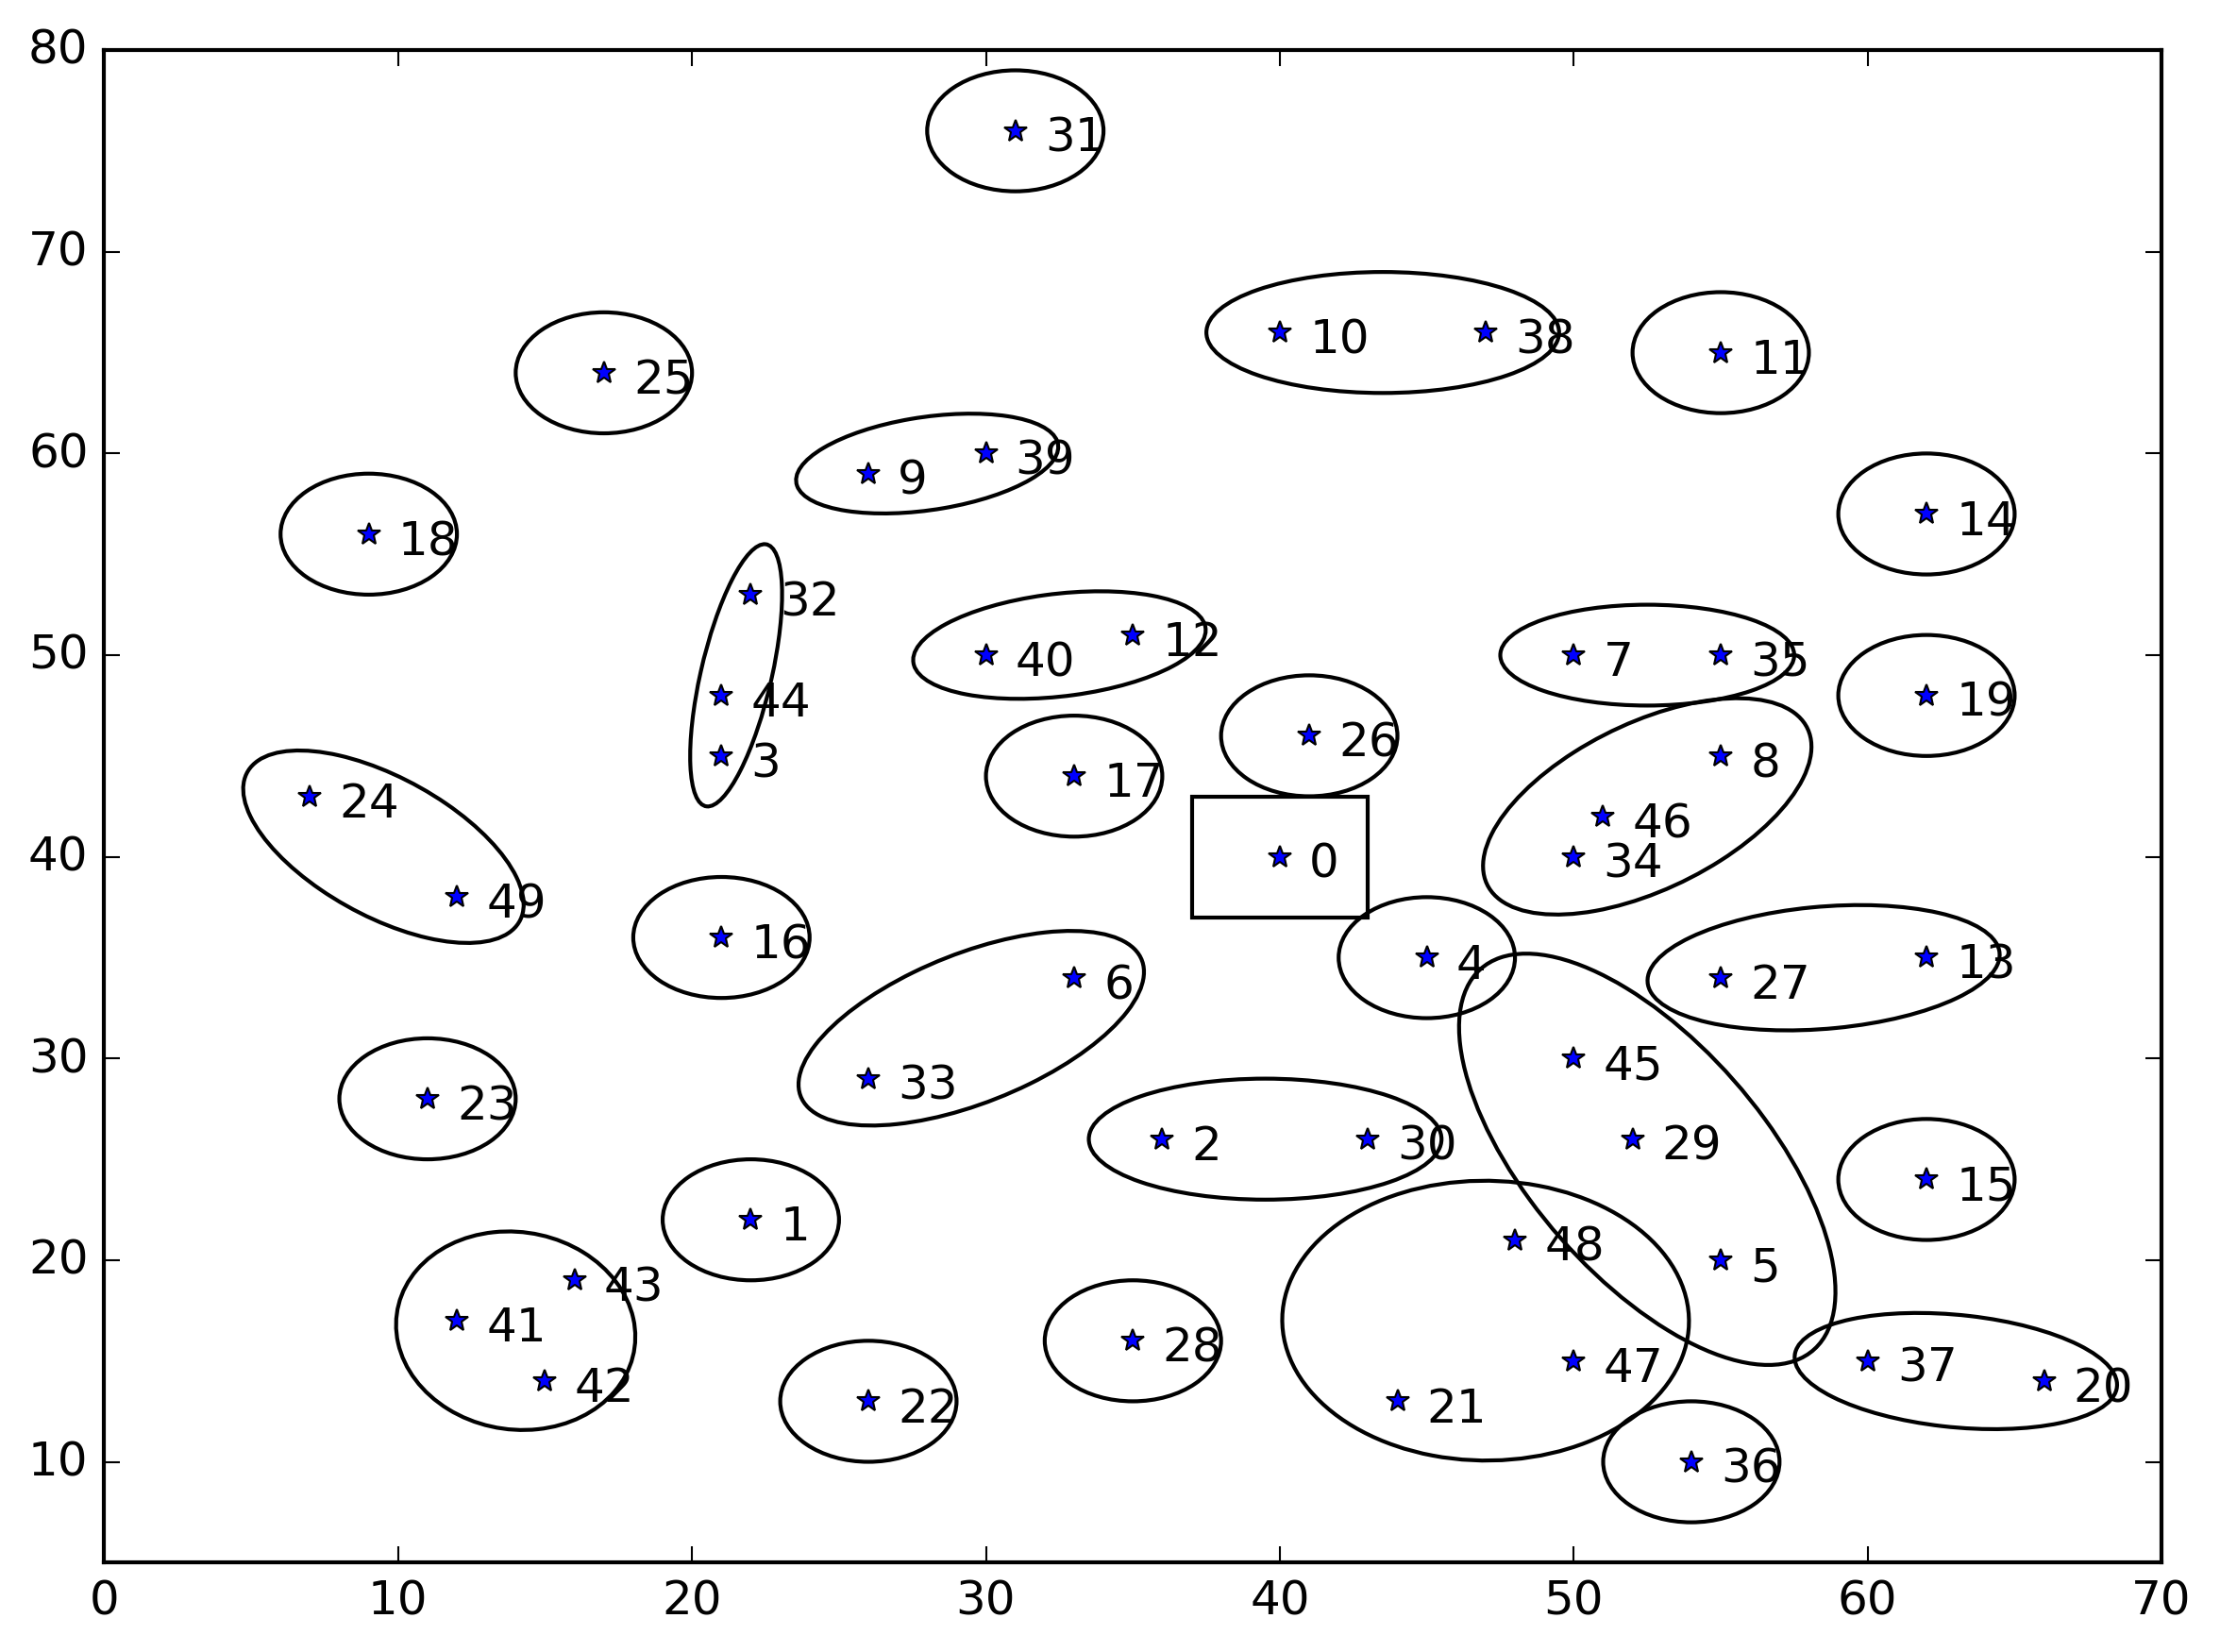
\includegraphics[width=0.45\textwidth]{P-n50-k10-c30_map.png}
%\label{fig:plot_11}}
%\quad
%\subfloat[Optimal solution (objective = 417.742)]{%
%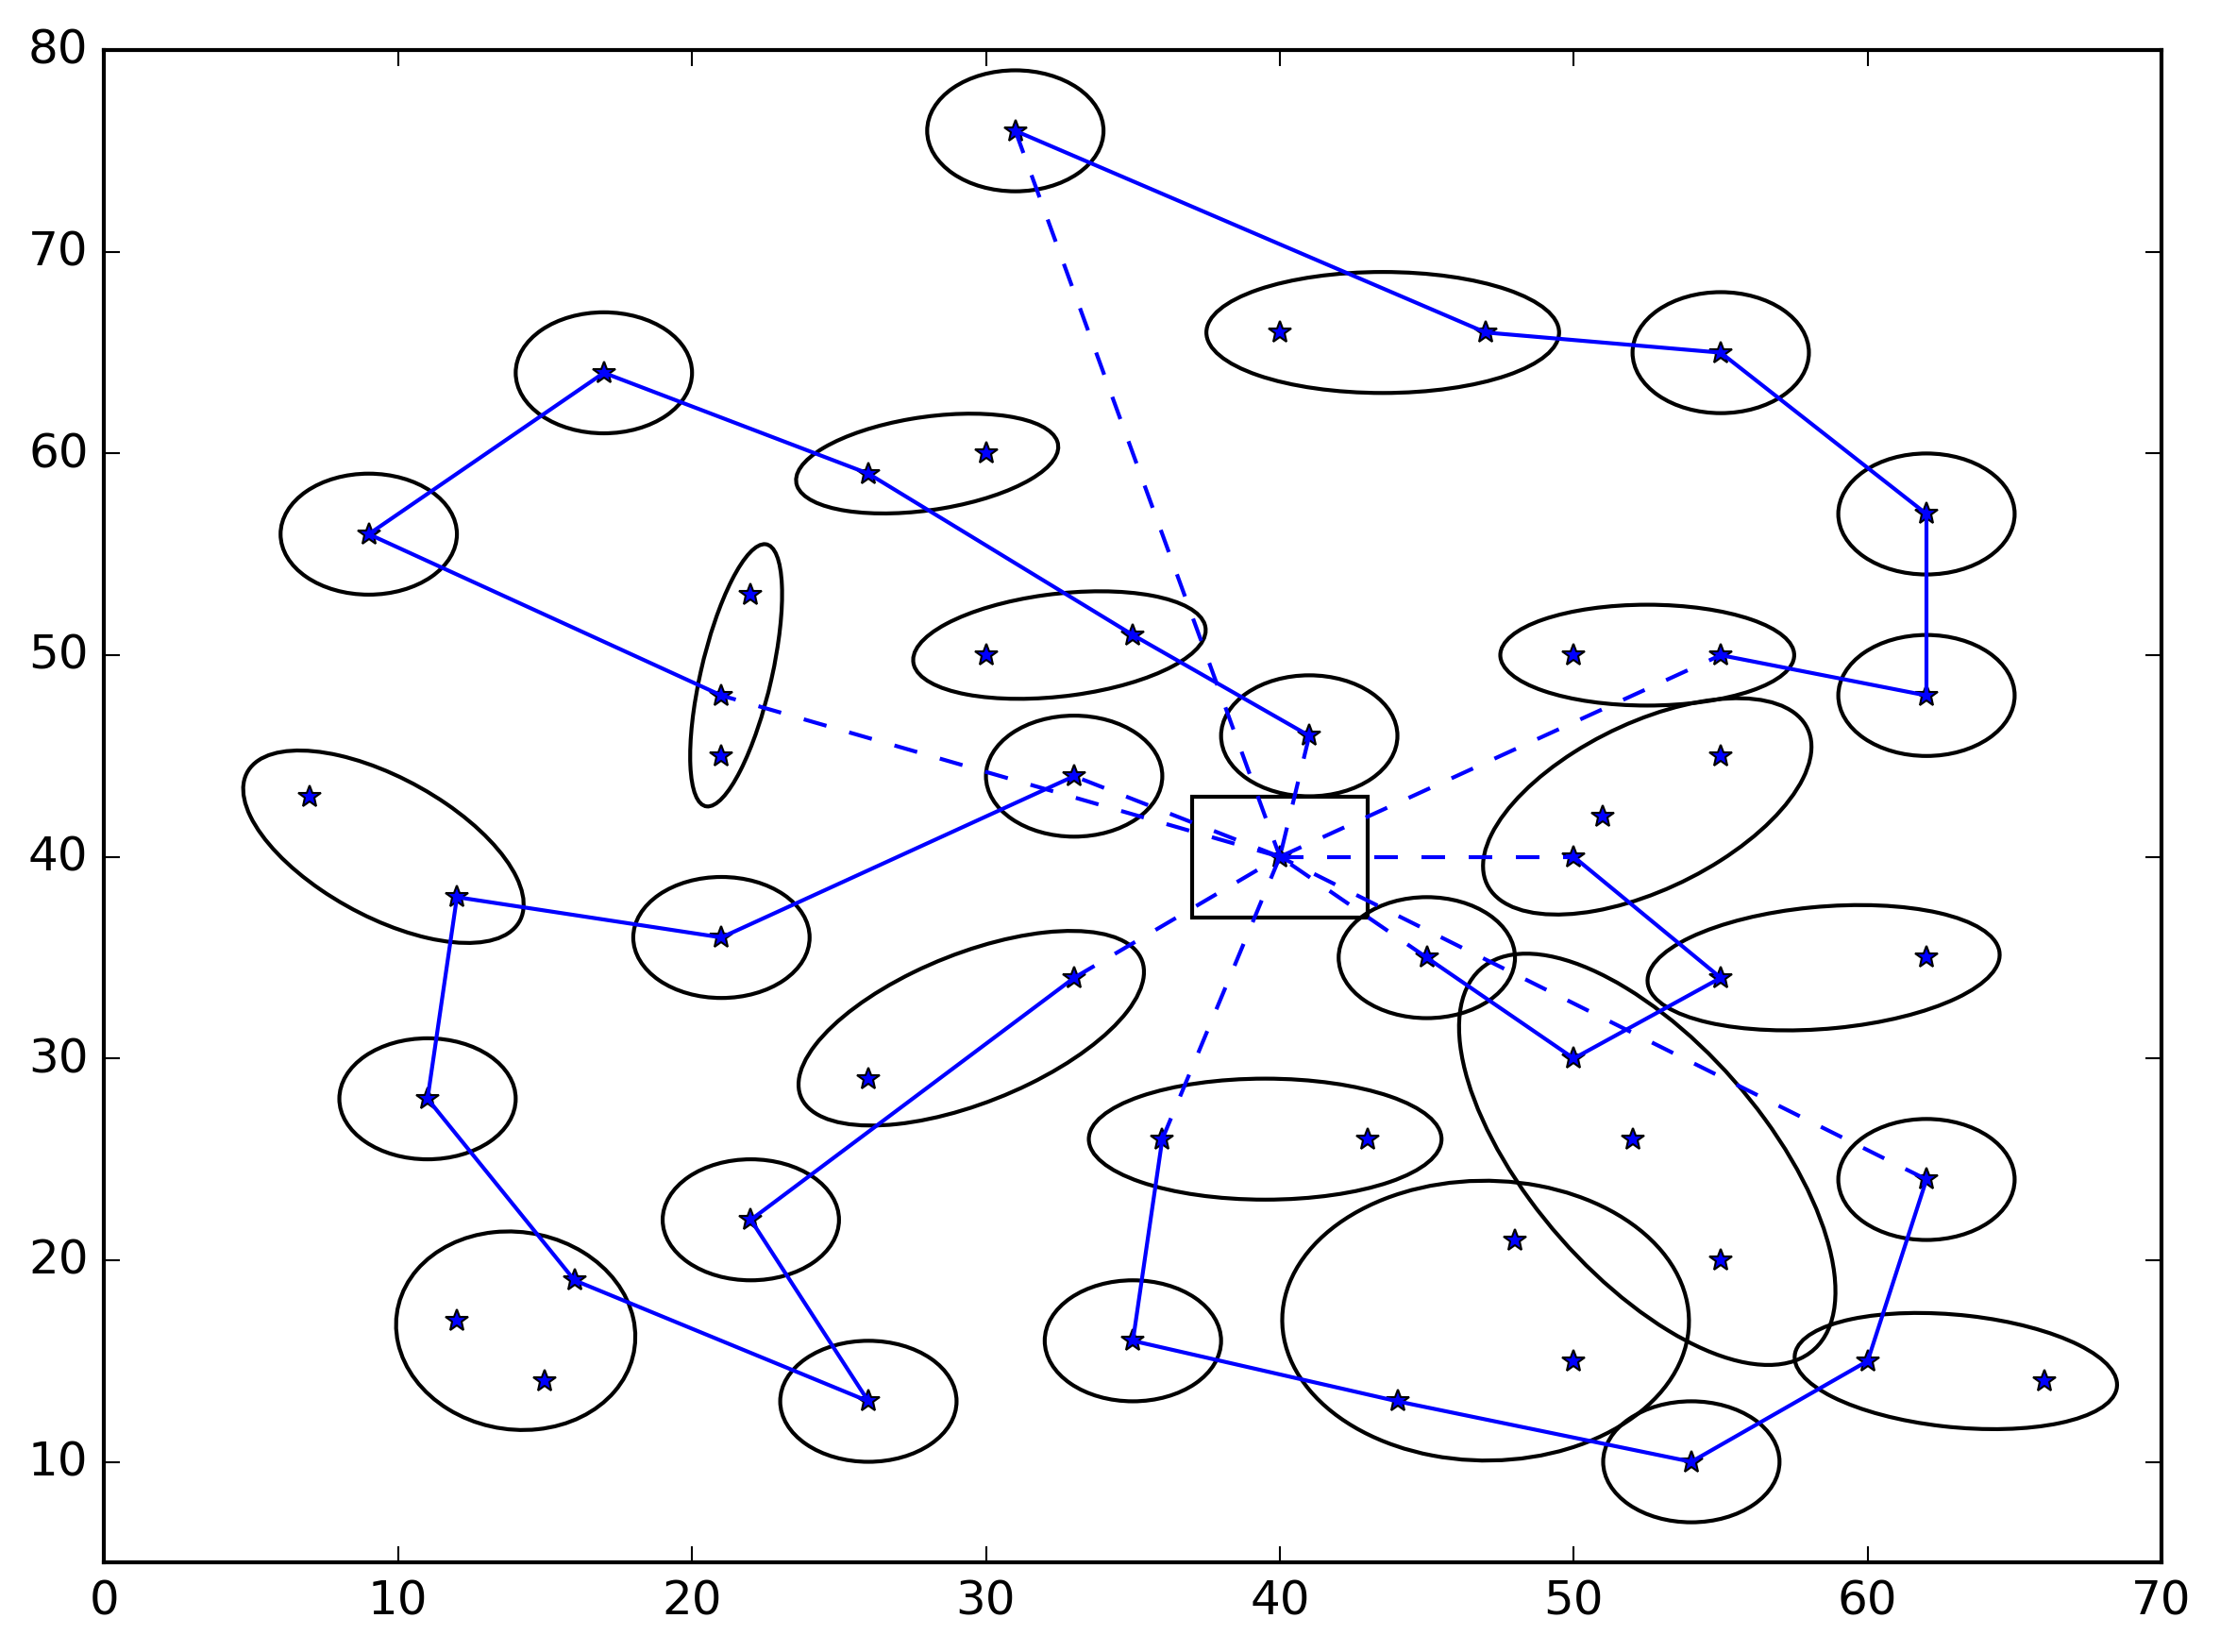
\includegraphics[width=0.45\textwidth]{P-n50-k10-c30_flow_n50_k31_m5_Q200_TL150_optimum.png}
%\label{fig:plots_12}}
%\caption{\texttt{P-n50-k10} (clustered)}
%\label{fig:P-n50-k10-sol}
%\end{figure}
%
%\begin{figure}[htbp]
%\centering
%\subfloat[Customer clusters]{%
%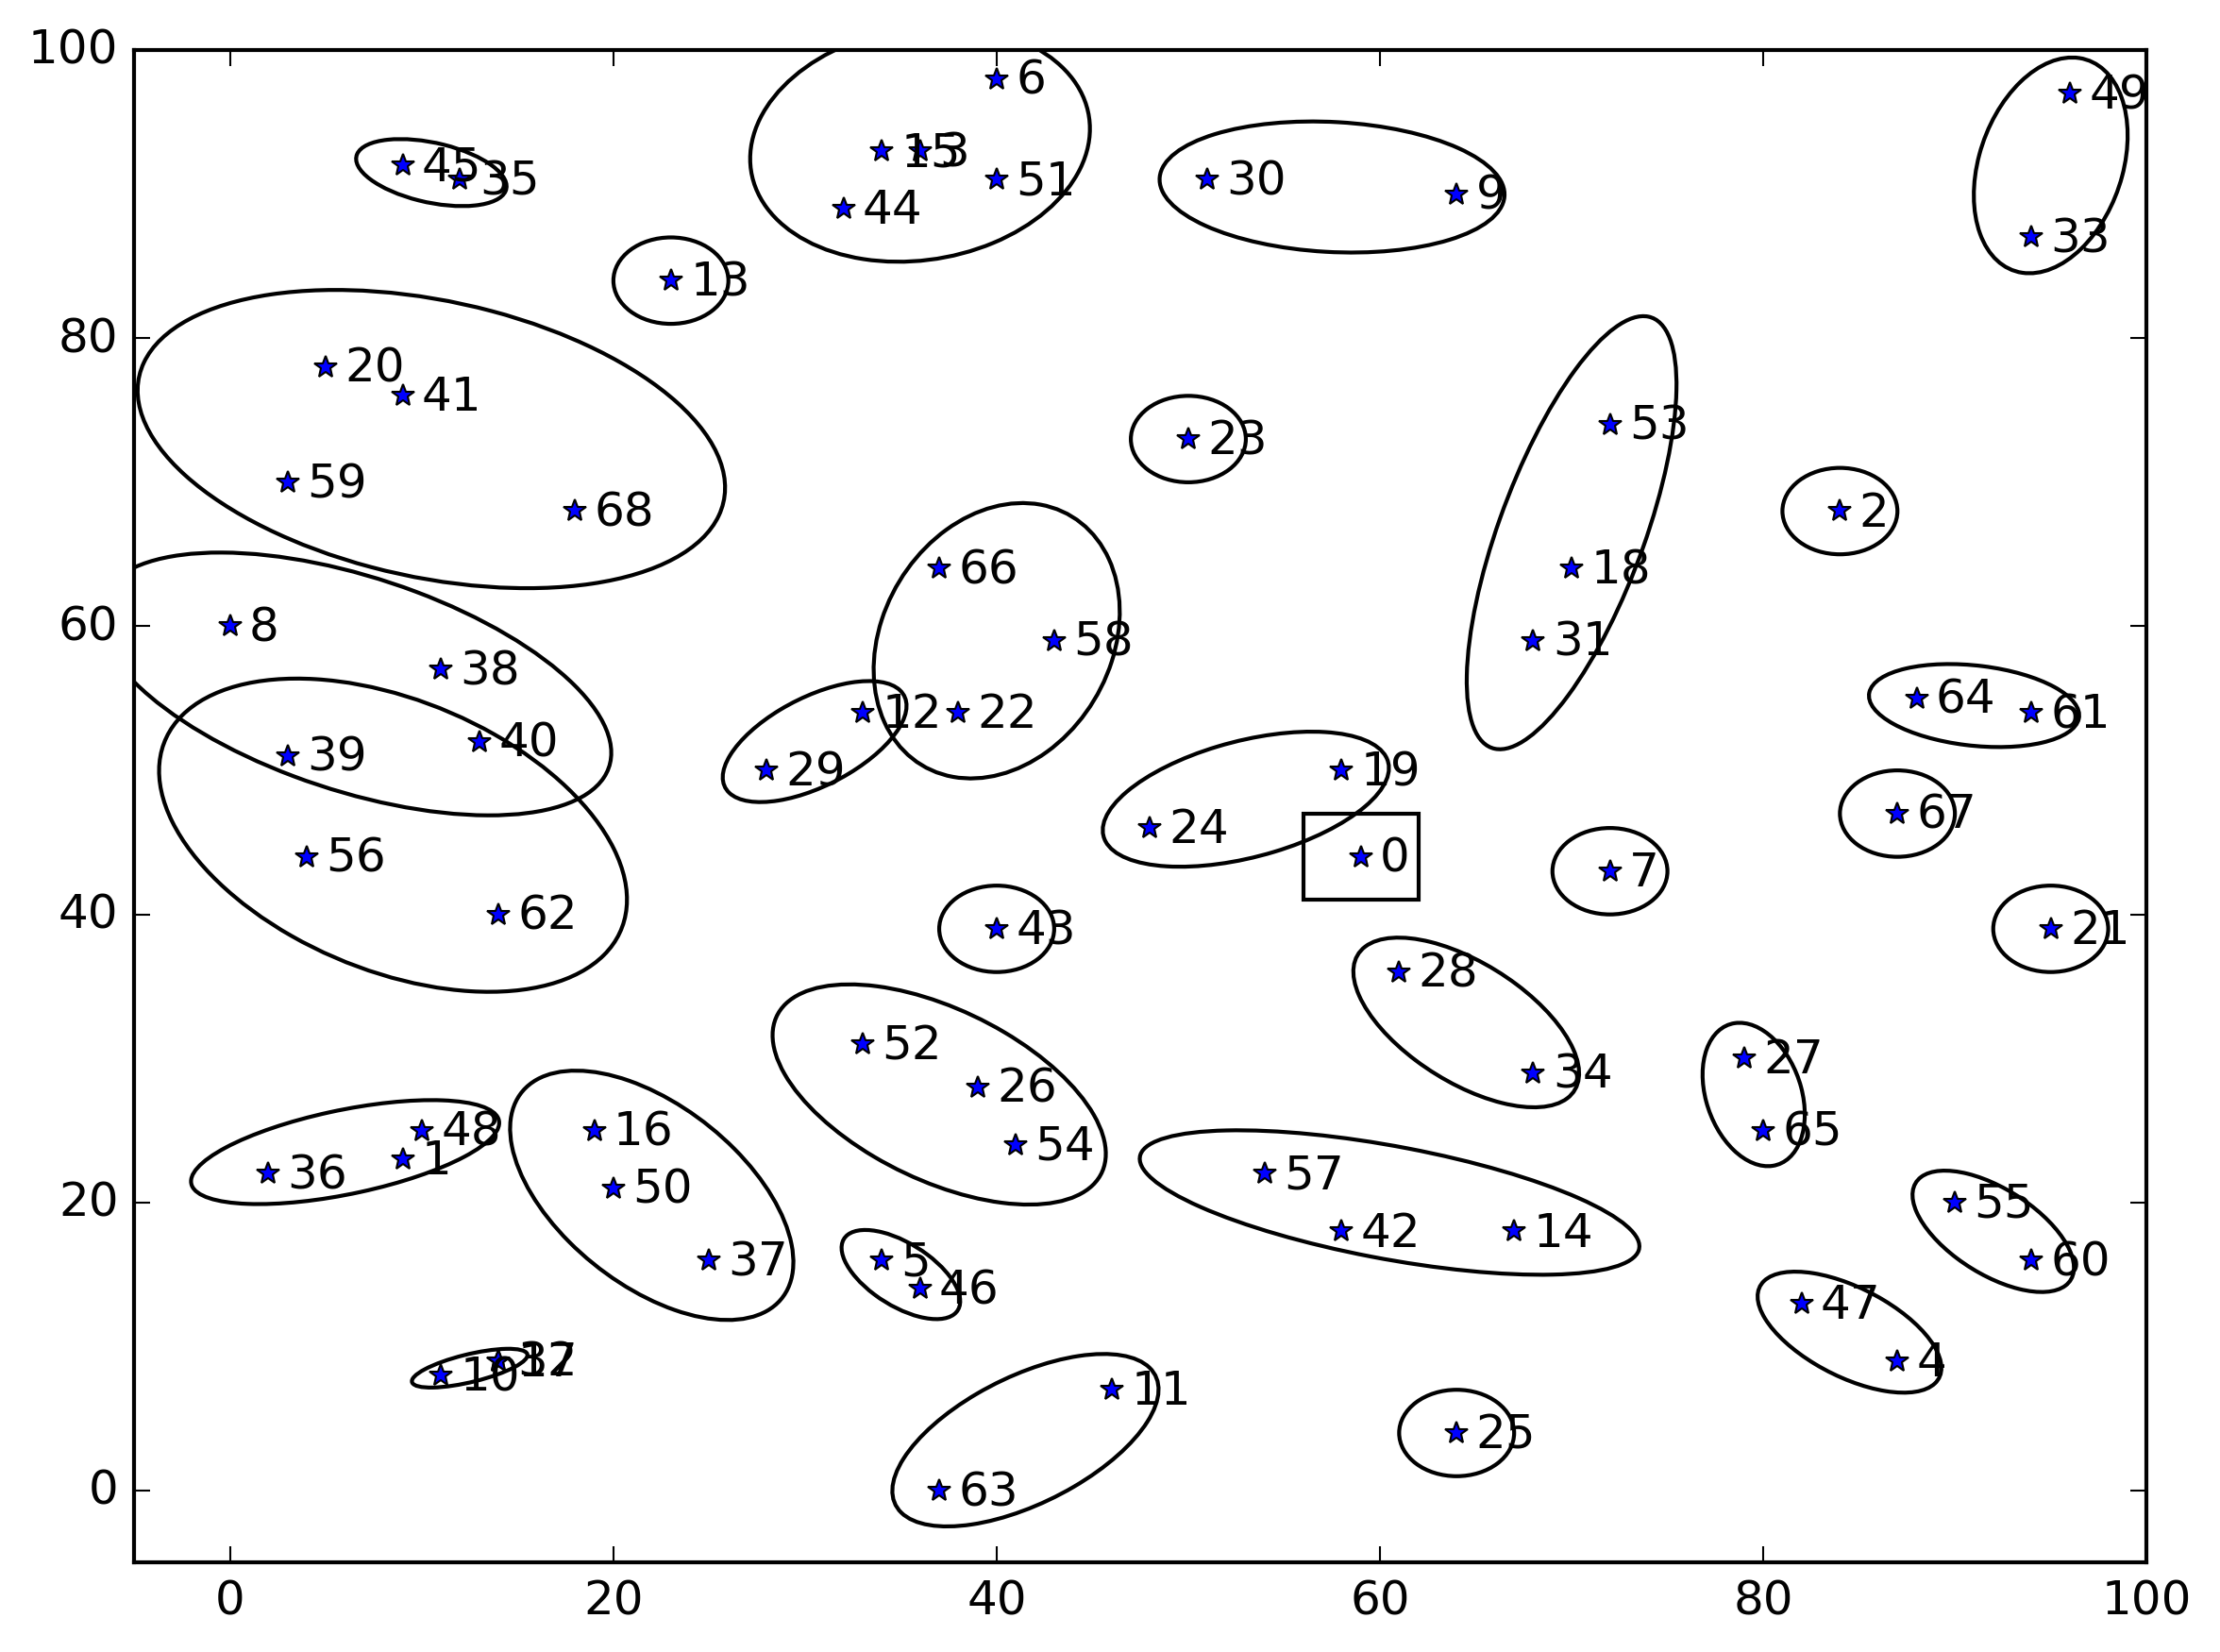
\includegraphics[width=0.45\textwidth]{A-n69-k9-c31_map.png}
%\label{fig:plot_11}}
%\quad
%\subfloat[Optimal solution (objective = 756.131)]{%
%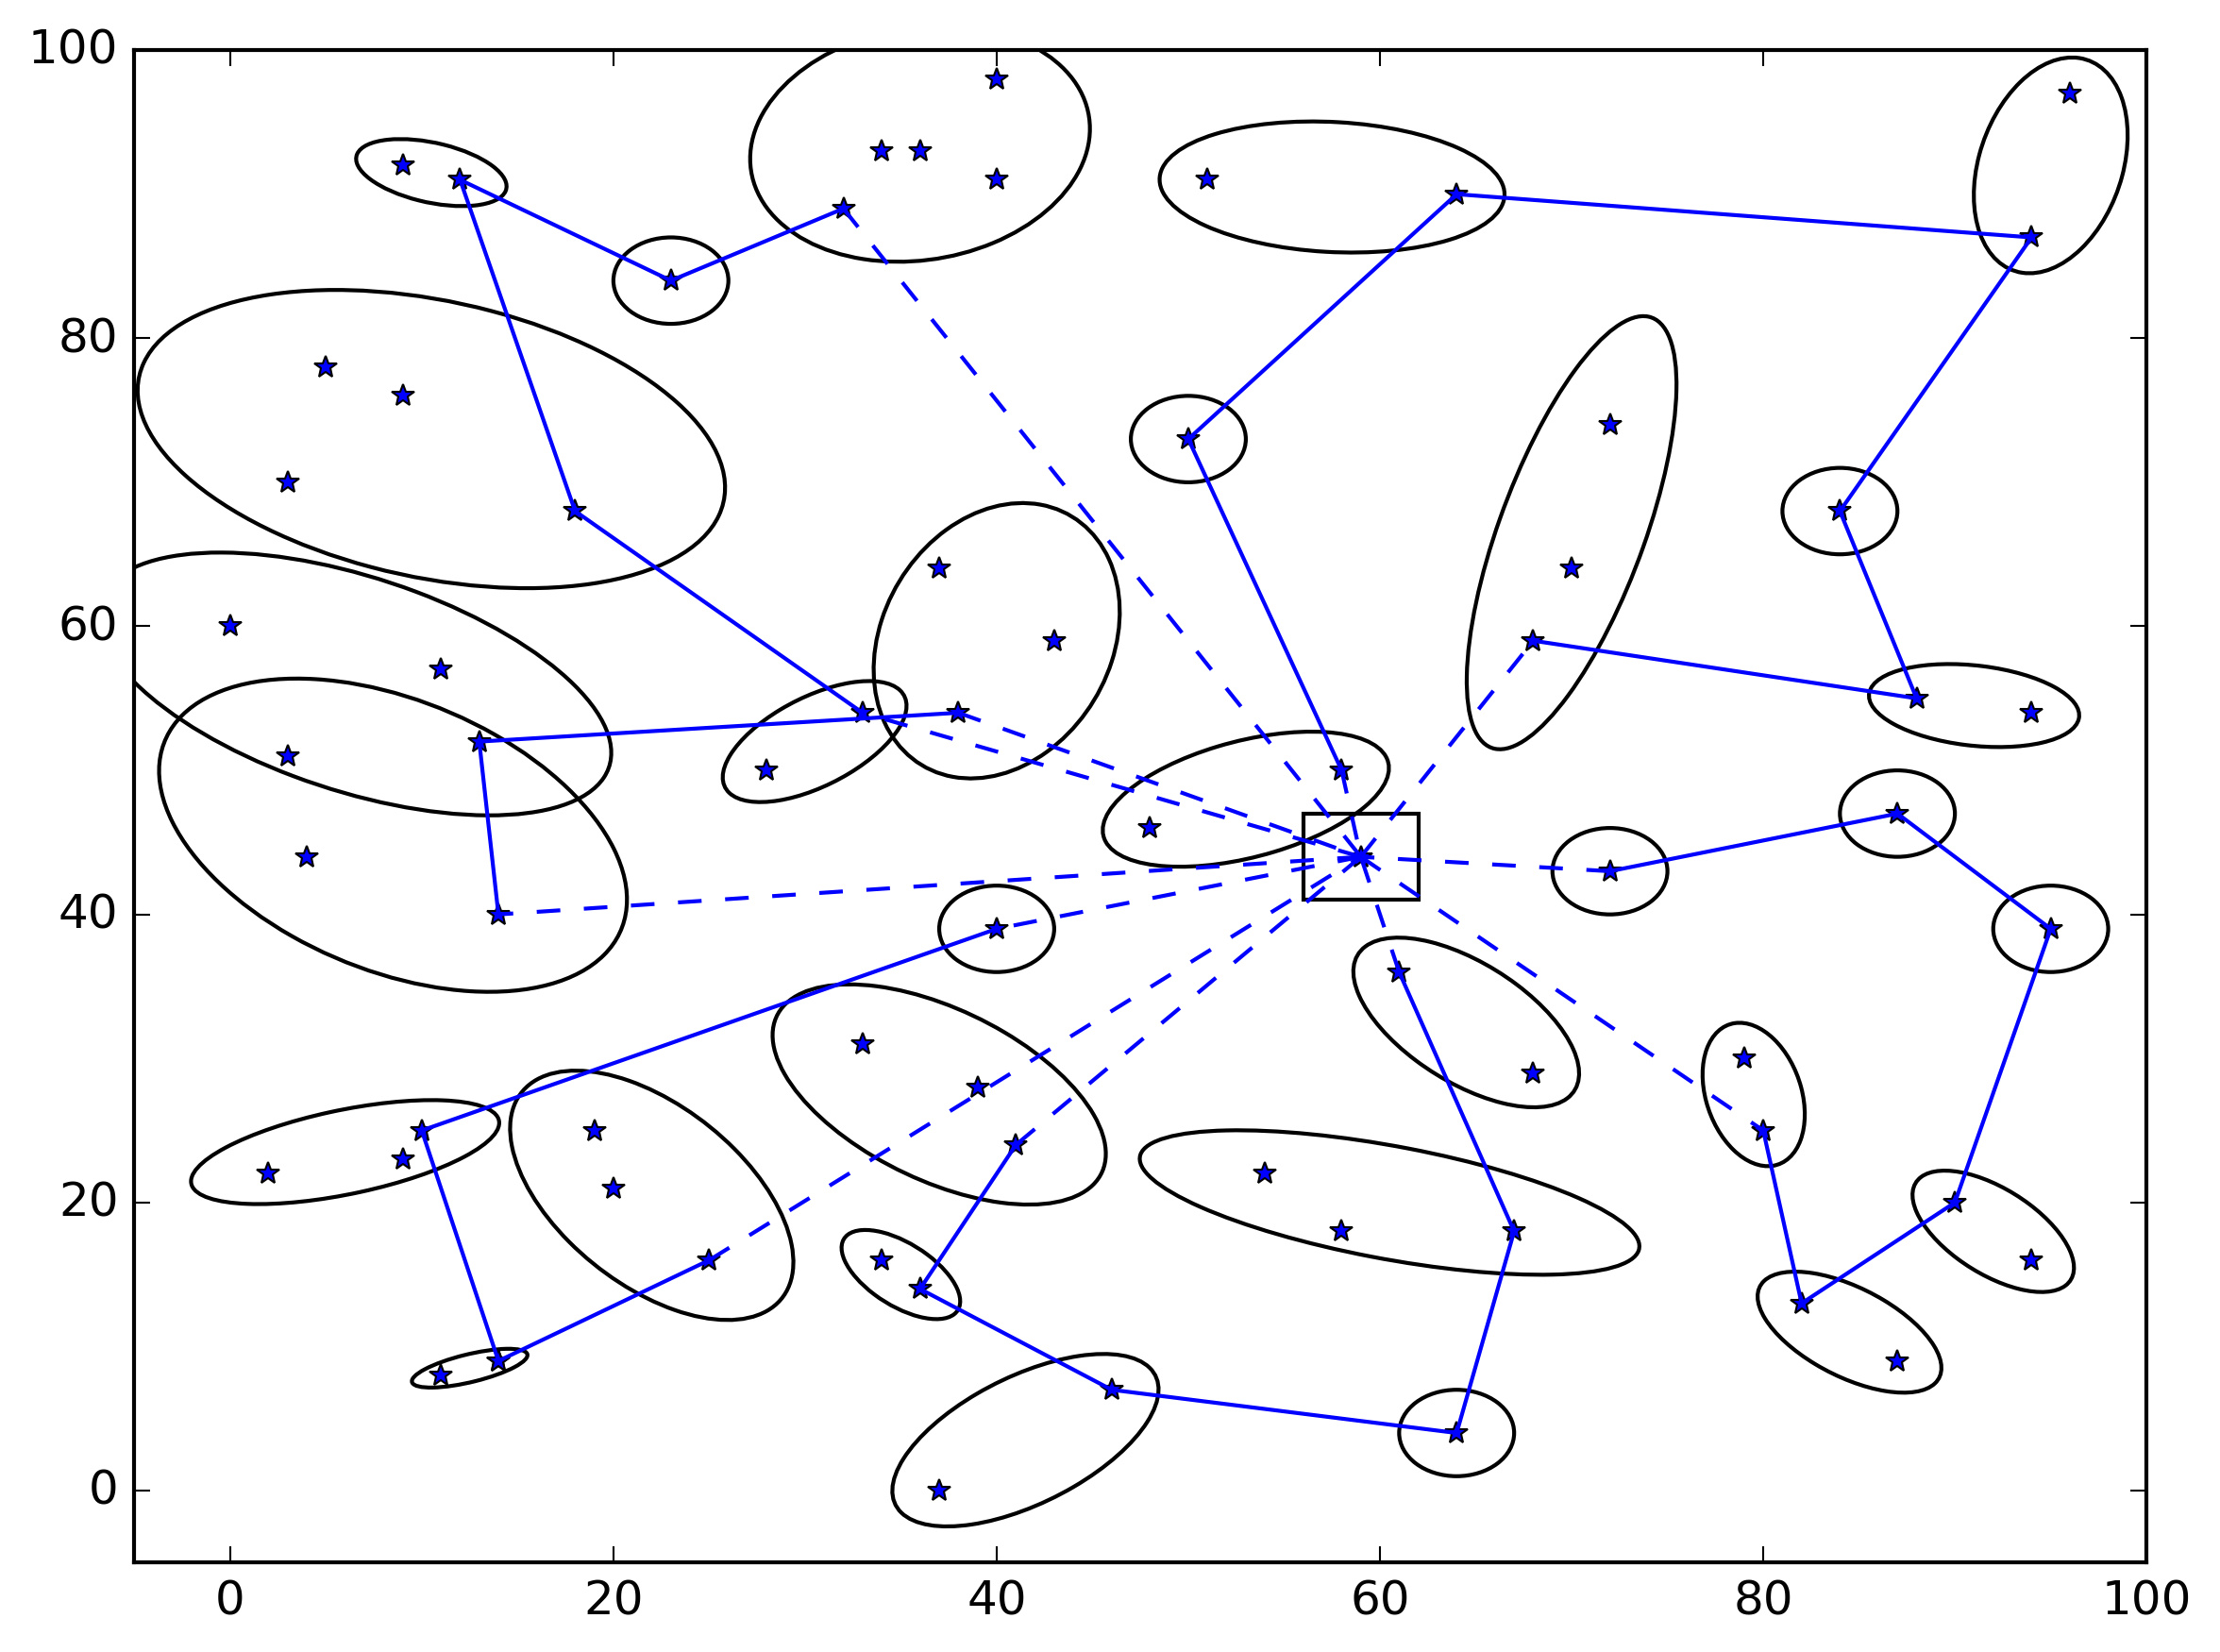
\includegraphics[width=0.45\textwidth]{A-n69-k9-c31_flow_n69_k32_m6_Q150_TL240_map.png}
%\label{fig:plots_12}}
%\caption{\texttt{A-n69-k9} (clustered)}
%\label{fig:A-n69-k9-sol}
%\end{figure}
%
%\section{Conclusions}
%Two MILP formulations of the generalized vehicle routing problem (GVRP) were studied. The number of variables and constraints is a polynomial function of the number of customers for both the formulations. 
%Two formulations were defined: the first had auxiliary variables defined based on the customers (node-based) where as the second had auxiliary variables defined based on arcs between customers (flow-based). 
%
%Three new instances were generated by clustering benchmark instances for the capacitated vehicle routing problem (CVRP). Computational studies were conducted to compare the node-based and flow-based formulations.
%The flow-based formulation was proved to have better computational properties as compared to the node-based formulation for all instances under consideration. Two of the new instances were solved to optimality using the superior flow-based formulation. 
%
%\begin{figure}[htbp]
%\centering
%\subfloat[Customer clusters]{%
%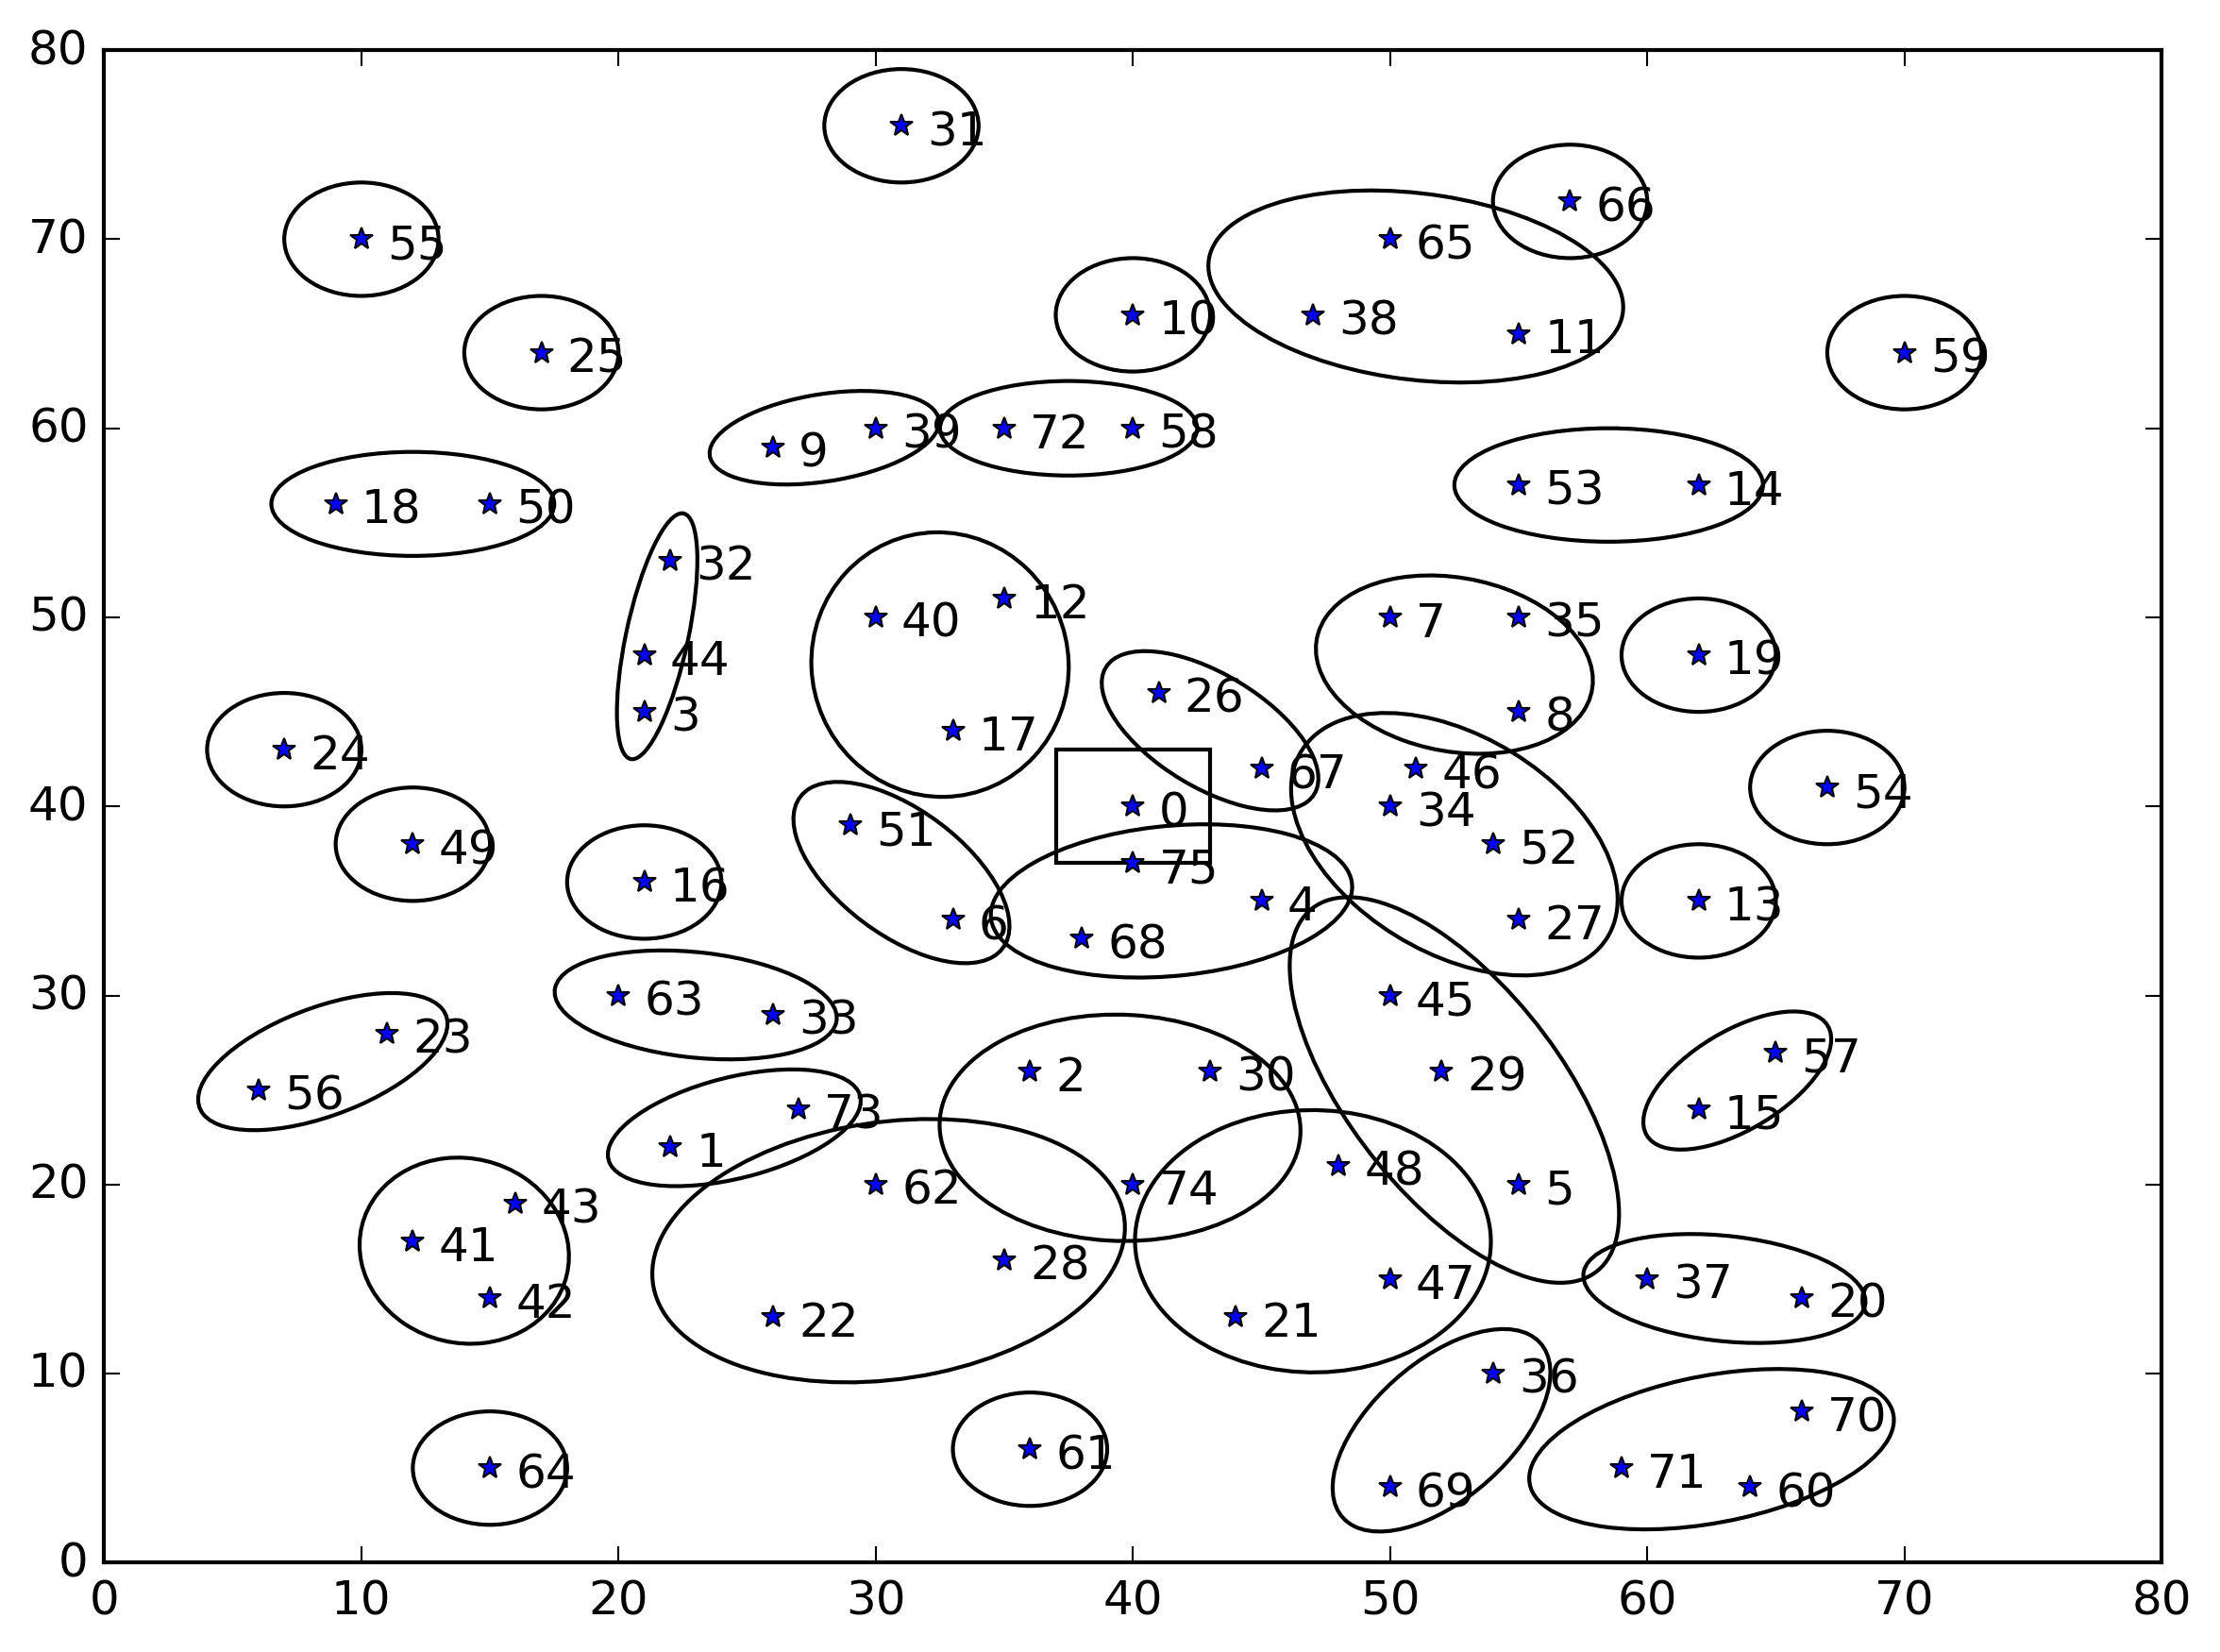
\includegraphics[width=0.45\textwidth]{P-n76-k5-c38_map.png}
%\label{fig:plot_11}}
%\quad
%\subfloat[Best known solution (objective = 500.955)]{%
%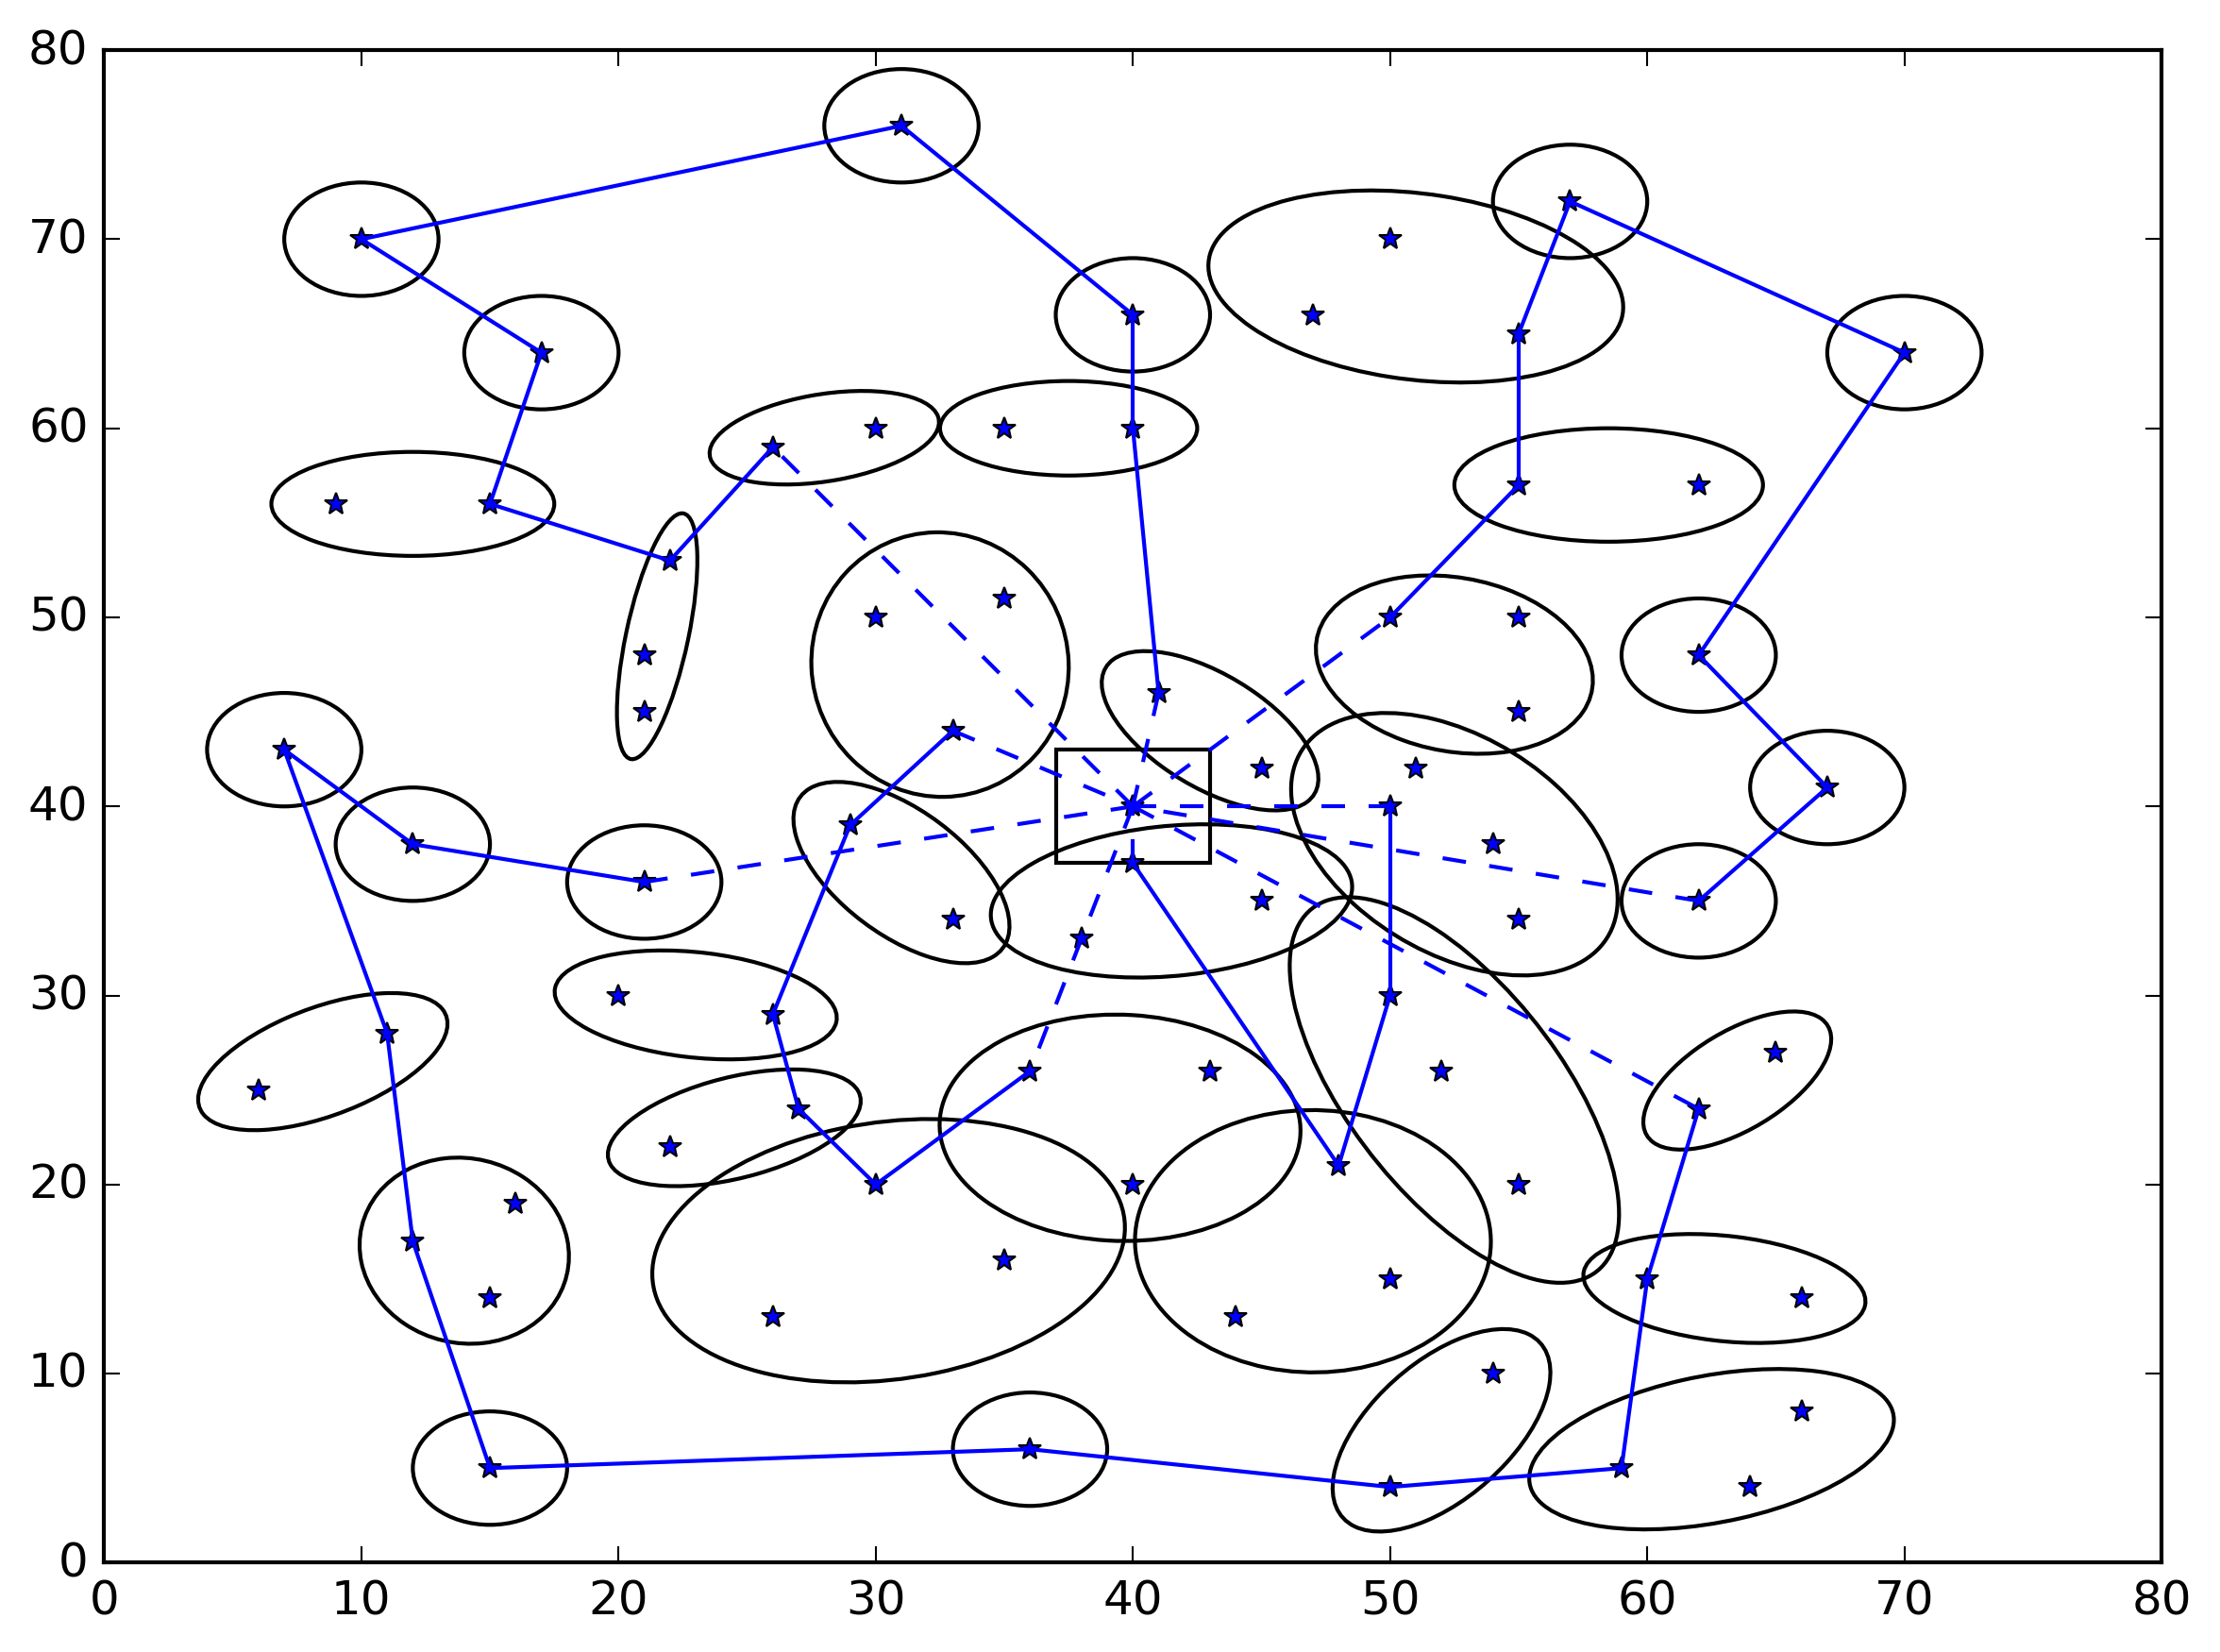
\includegraphics[width=0.45\textwidth]{P-n76-k5-c38_flow_n76_k39_m5_Q280_TL480_map.png}
%\label{fig:plots_12}}
%\caption{\texttt{P-n76-k5} (clustered)}
%\label{fig:P-n76-k5-c38-sol }
%\end{figure}

\newpage
%\nocite{*}  %% uncomment to include all references in bib file
\bibliographystyle{ICTv3}
\bibliography{Proposal_bib}

\newpage

%\section*{Appendix}
%
%\renewcommand{\thefigure}{A\arabic{figure}}
%\setcounter{figure}{0}


%\begin{figure}[htbp]
%\centering
%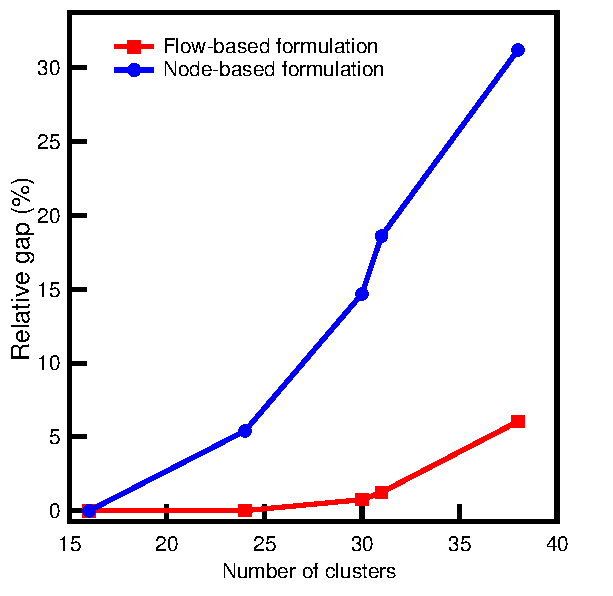
\includegraphics[width=0.6\textwidth]{cok.pdf}
%\caption{asfda}
%\label{fig:w}
%\end{figure}

\end{document}